\documentclass[a4paper,11pt,oneside]{memoir}

% Castellano
\usepackage[spanish]{babel}
\selectlanguage{spanish}
\usepackage[utf8]{inputenc}
\usepackage{placeins}
\usepackage{subfloat}
\usepackage{subfig}
\usepackage{eurosym} 

\RequirePackage{booktabs}
\RequirePackage[table]{xcolor}
\RequirePackage{xtab}
\RequirePackage{multirow}

% Links\tablaSmall{
\usepackage[colorlinks]{hyperref}
\hypersetup{
	allcolors = {red}
}

% Ecuaciones
\usepackage{amsmath}

% Rutas de fichero / paquete
\newcommand{\ruta}[1]{{\sffamily #1}}

% Párrafos
\nonzeroparskip


% Imagenes
\usepackage{graphicx}
\newcommand{\imagen}[2]{
	\begin{figure}[!h]
		\centering
		\includegraphics[width=0.9\textwidth]{#1}
		\caption{#2}\label{fig:#1}
	\end{figure}
	\FloatBarrier
}

\newcommand{\imagenflotante}[2]{
	\begin{figure}%[!h]
		\centering
		\includegraphics[width=0.9\textwidth]{#1}
		\caption{#2}\label{fig:#1}
	\end{figure}
}



% El comando \figura nos permite insertar figuras comodamente, y utilizando
% siempre el mismo formato. Los parametros son:
% 1 -> Porcentaje del ancho de página que ocupará la figura (de 0 a 1)
% 2 --> Fichero de la imagen
% 3 --> Texto a pie de imagen
% 4 --> Etiqueta (label) para referencias
% 5 --> Opciones que queramos pasarle al \includegraphics
% 6 --> Opciones de posicionamiento a pasarle a \begin{figure}
\newcommand{\figuraConPosicion}[6]{%
  \setlength{\anchoFloat}{#1\textwidth}%
  \addtolength{\anchoFloat}{-4\fboxsep}%
  \setlength{\anchoFigura}{\anchoFloat}%
  \begin{figure}[#6]
    \begin{center}%
      \Ovalbox{%
        \begin{minipage}{\anchoFloat}%
          \begin{center}%
            \includegraphics[width=\anchoFigura,#5]{#2}%
            \caption{#3}%
            \label{#4}%
          \end{center}%
        \end{minipage}
      }%
    \end{center}%
  \end{figure}%
}

%
% Comando para incluir imágenes en formato apaisado (sin marco).
\newcommand{\figuraApaisadaSinMarco}[5]{%
  \begin{figure}%
    \begin{center}%
    \includegraphics[angle=90,height=#1\textheight,#5]{#2}%
    \caption{#3}%
    \label{#4}%
    \end{center}%
  \end{figure}%
}
% Para las tablas
\newcommand{\otoprule}{\midrule [\heavyrulewidth]}
%
% Nuevo comando para tablas pequeñas (menos de una página).
\newcommand{\tablaSmall}[5]{%
 \begin{table}[htb]
  \begin{center}
   \rowcolors {2}{gray!35}{}
   \begin{tabular}{#2}
    \toprule
    #4
    \otoprule
    #5
    \bottomrule
   \end{tabular}
   \caption{#1}
   \label{tabla:#3}
  \end{center}
 \end{table}
}

%
% Nuevo comando para tablas pequeñas (menos de una página).
\newcommand{\tablaSmallSinColores}[5]{%
 \begin{table}[H]
  \begin{center}
   \begin{tabular}{#2}
    \toprule
    #4
    \otoprule
    #5
    \bottomrule
   \end{tabular}
   \caption{#1}
   \label{tabla:#3}
  \end{center}
 \end{table}
}

\newcommand{\tablaApaisadaSmall}[5]{%
\begin{landscape}
  \begin{table}
   \begin{center}
    \rowcolors {2}{gray!35}{}
    \begin{tabular}{#2}
     \toprule
     #4
     \otoprule
     #5
     \bottomrule
    \end{tabular}
    \caption{#1}
    \label{tabla:#3}
   \end{center}
  \end{table}
\end{landscape}
}

%
% Nuevo comando para tablas grandes con cabecera y filas alternas coloreadas en gris.
\newcommand{\tabla}[6]{%
  \begin{center}
    \tablefirsthead{
      \toprule
      #5
      \otoprule
    }
    \tablehead{
      \multicolumn{#3}{l}{\small\sl continúa desde la página anterior}\\
      \toprule
      #5
      \otoprule
    }
    \tabletail{
      \hline
      \multicolumn{#3}{r}{\small\sl continúa en la página siguiente}\\
    }
    \tablelasttail{
      \hline
    }
    \bottomcaption{#1}
    \rowcolors {2}{gray!35}{}
    \begin{xtabular}{#2}
      #6
      \bottomrule
    \end{xtabular}
    \label{tabla:#4}
  \end{center}
}

%
% Nuevo comando para tablas grandes con cabecera.
\newcommand{\tablaSinColores}[6]{%
  \begin{center}
    \tablefirsthead{
      \toprule
      #5
      \otoprule
    }
    \tablehead{
      \multicolumn{#3}{l}{\small\sl continúa desde la página anterior}\\
      \toprule
      #5
      \otoprule
    }
    \tabletail{
      \hline
      \multicolumn{#3}{r}{\small\sl continúa en la página siguiente}\\
    }
    \tablelasttail{
      \hline
    }
    \bottomcaption{#1}
    \begin{xtabular}{#2}
      #6
      \bottomrule
    \end{xtabular}
    \label{tabla:#4}
  \end{center}
}

%
% Nuevo comando para tablas grandes sin cabecera.
\newcommand{\tablaSinCabecera}[5]{%
  \begin{center}
    \tablefirsthead{
      \toprule
    }
    \tablehead{
      \multicolumn{#3}{l}{\small\sl continúa desde la página anterior}\\
      \hline
    }
    \tabletail{
      \hline
      \multicolumn{#3}{r}{\small\sl continúa en la página siguiente}\\
    }
    \tablelasttail{
      \hline
    }
    \bottomcaption{#1}
  \begin{xtabular}{#2}
    #5
   \bottomrule
  \end{xtabular}
  \label{tabla:#4}
  \end{center}
}



\definecolor{cgoLight}{HTML}{EEEEEE}
\definecolor{cgoExtralight}{HTML}{FFFFFF}

%
% Nuevo comando para tablas grandes sin cabecera.
\newcommand{\tablaSinCabeceraConBandas}[5]{%
  \begin{center}
    \tablefirsthead{
      \toprule
    }
    \tablehead{
      \multicolumn{#3}{l}{\small\sl continúa desde la página anterior}\\
      \hline
    }
    \tabletail{
      \hline
      \multicolumn{#3}{r}{\small\sl continúa en la página siguiente}\\
    }
    \tablelasttail{
      \hline
    }
    \bottomcaption{#1}
    \rowcolors[]{1}{cgoExtralight}{cgoLight}

  \begin{xtabular}{#2}
    #5
   \bottomrule
  \end{xtabular}
  \label{tabla:#4}
  \end{center}
}


















\graphicspath{ {./img/} }

% Capítulos
\chapterstyle{bianchi}
\newcommand{\capitulo}[2]{
	\setcounter{chapter}{#1}
	\setcounter{section}{0}
	\chapter*{#2}
	\addcontentsline{toc}{chapter}{#2}
	\markboth{#2}{#2}
}

% Apéndices
\renewcommand{\appendixname}{Apéndice}
\renewcommand*\cftappendixname{\appendixname}

\newcommand{\apendice}[1]{
	%\renewcommand{\thechapter}{A}
	\chapter{#1}
}

\renewcommand*\cftappendixname{\appendixname\ }

% Formato de portada
\makeatletter
\usepackage{xcolor}
\newcommand{\tutor}[1]{\def\@tutor{#1}}
\newcommand{\cotutor}[1]{\def\@cotutor{#1}}
\newcommand{\course}[1]{\def\@course{#1}}
\definecolor{cpardoBox}{HTML}{E6E6FF}
\def\maketitle{
  \null
  \thispagestyle{empty}
  % Cabecera ----------------
\noindent
\includegraphics[width=\textwidth]{cabecera}\vspace{1cm}%
  \vfill
  % Título proyecto y escudo informática ----------------
  \colorbox{cpardoBox}{%
    \begin{minipage}{.8\textwidth}
      \vspace{.5cm}\Large
      \begin{center}
      \textbf{TFG del Grado en Ingeniería Informática}\vspace{.6cm}\\
      \textbf{\LARGE\@title{}}
      \end{center}
      \vspace{.2cm}
    \end{minipage}

  }%
  \hfill\begin{minipage}{.20\textwidth}
    
\includegraphics[width=\textwidth]{escudoInfor}
  \end{minipage}
  \vfill
  % Datos de alumno, curso y tutores ------------------
  \begin{center}%
  {%
    \noindent\LARGE
    Presentado por \@author{}\\ 
    en Universidad de Burgos --- \@date{}\\
    Tutores: \@tutor{}\\
   	y \@cotutor{}\\
  }%
  \end{center}%
  \null
  \cleardoublepage
  }
\makeatother


% Datos de portada
\title{Escaner de tiques de compra}
\author{Roberto Miranda Pérez}
\tutor{Dr.José Francisco Diez Pastor}
\cotutor{Dr.Raúl Marticorena Sánchez}
\date{\today}

\setcounter{secnumdepth}{5}
\begin{document}

\maketitle



\null\cleardoublepage


%%%%%%%%%%%%%%%%%%%%%%%%%%%%%%%%%%%%%%%%%%%%%%%%%%%%%%%%%%%%%%%%%%%%%%%%%%%%%%%%%%%%%%%%
\pagestyle{empty}


\noindent
\includegraphics[width=\textwidth]{cabecera}\vspace{1cm}

\noindent D.José Francisco Diez Pastor, profesor del departamento de nombre departamento, área de nombre área.

\noindent Expone:

\noindent Que el alumno D.Roberto Miranda Pérez , con DNI 71298459T, ha realizado el Trabajo final de Grado en Ingeniería Informática titulado Escaner de tiques de compra. 

\noindent Y que dicho trabajo ha sido realizado por el alumno bajo la dirección del que suscribe, en virtud de lo cual se autoriza su presentación y defensa.

\begin{center} %\large
En Burgos, {\large \today}
\end{center}

\vfill\vfill\vfill

% Author and supervisor
\begin{minipage}{0.45\textwidth}
\begin{flushleft} %\large
Vº. Bº. del Tutor:\\[2cm]
D. nombre tutor
\end{flushleft}
\end{minipage}
\hfill
\begin{minipage}{0.45\textwidth}
\begin{flushleft} %\large
Vº. Bº. del Tutor:\\[2cm]
D. nombre tutor
\end{flushleft}
\end{minipage}
\hfill

\vfill



% para casos con solo un tutor comentar lo anterior
% y descomentar lo siguiente
%Vº. Bº. del Tutor:\\[2cm]
%D. nombre tutor


\null\cleardoublepage
\null\cleardoublepage




\frontmatter

% Abstract en castellano
\renewcommand*\abstractname{Resumen}
\begin{abstract}
En el presente trabajo se desarrolla  un sistema capaz de obtener los productos(nombre , precio, cantidad) a partir de una imagen de un tique de compra.
El problema se aborda mediante la manipulación de la imagen para después transformarla en texto mediante un proceso llamado \textit{OCR}, o en castellano \textit{reconocimiento óptico de caracteres}, que permita almacenar su información en un dispositivo móvil.
La automatización de este proceso,permite el ahorro de tiempo y esfuerzo para los usuarios que desean llevar una contabilidad electrónica de sus gastos, ya que hoy en día, el proceso para almacenar estos tiques se debe realizar de forma manual.

El presente trabajo ha sido desarrollado en dos partes, una parte cliente que se encarga de la toma de imágenes y mostrar la información al usuario, y una parte servidor, la cual se encarga del procesado de la imagen y su transformación a texto para después enviarla al cliente.
\end{abstract}

\renewcommand*\abstractname{Descriptores}
\begin{abstract}
Android, Cliente,Servidor, OCR, Tesseract, Distancia de Levenshtein, Linea de tique.
\end{abstract}

\clearpage

% Abstract en inglés
\renewcommand*\abstractname{Abstract}
\begin{abstract}
The present project develops a system able to obtain the name,price and quantity of products from an image of a purchase's ticket.
This question is approached by means of the manipulation of the image then, this image is transformed into a text throught a process called \textit{OCR}, or in spanish \textit{reconocimiento óptico de caracteres}, witch allows to store its information.
This process of automation saves time and effort to de users who wish to carry out and electronic accountancy of their expenses, since today the process to store these tickets has to be done manually.
The present project has been developed in two different parts, the firest part is called \textit{client} which is in charge of the image's taking and showing the information to the user, the second part is called \textit{server}. The server processes the image and its transformation into a text that is then sent to the client.  
\end{abstract}

\renewcommand*\abstractname{Keywords}
\begin{abstract}
Android, Client ,Server, OCR, Tesseract, Levenshtein distance, Ticket line.
\end{abstract}

\clearpage

% Indices
\tableofcontents

\clearpage

\listoffigures

\clearpage

\listoftables

\clearpage

\mainmatter
\capitulo{1}{Introducción}

En la era de la información que nos encontramos, donde todos los servicios se encuentran a click de ratón, el papel impreso está destinado a desaparecer. Sin embargo el ser humano es precavido y tiende a guardar todos los datos, por ello en los últimos años se ha empezado a digitalizar  los viejos informes de papel organizados en archivadores y ser guardados en grandes bancos de datos, que permiten una organización mucho mas limpia y más eficaz a la hora de acceder y buscar estos datos.

 Cada día realizamos compras ya a sea a través de la pantalla de dispositivos electrónicos, o de una forma mas tradicional con el contacto cliente-vendedor. En todas estas transacciones se genera una factura o tique, siendo en estas ultimas en papel, los cuales guardamos en la cartera o en casa para poder realizar un control de nuestros gastos y si es posible ahorrar en futuras compras.
 
 Este tipo de documentos también pueden ser digitalizados, sin embargo con este proyecto se quiere ir un paso mas allá, permitiendo guardar en un sistema persistente de base de datos cada articulo o producto adquirido, de forma automática, lo que permitiría un ahorro considerable de tiempo del usuario a la hora de guardar y consultar sus gastos.
 
 Generalmente las aplicaciones de control de gastos que podemos encontrar en el mercado de aplicaciones, en el caso de Android, Google Play emplean un sistema manual de almacenamiento de los datos, lo que hace que el usuario generalmente deje de emplear este tipo de sistema, ya que por naturaleza, las personas somos perezosas.
 
 La automatización del guardado de estos datos no solo ahorraría tiempo al usuario, si no que todos estos datos almacenados seria de gran importancia para las grandes compañías que realizan estudios de mercado y tendencias de compra, por lo tanto tendría un gran valor económico.
 
 La realización del presente trabajo se encuentra  dentro del campo de la visión artificial,el cual, se centra en la obtención de los datos a partir de una imagen.
 
 
 

\capitulo{2}{Objetivos del proyecto}

Con este proyecto se pretende conseguir una aplicación para smartphones basados en el sistema operativo  Android, con la que se pueda llevar un seguimiento de los gastos realizados por el usuario a través de una foto al tique.

\subsection{Objetivos Específicos}
Los objetivos dados por los requisitos software para el desarrollo del presente trabajo son los siguientes: 
\begin{itemize}
	\item Desarrollo de una aplicación para smartphones que permita llevar un historial de las compras realizadas por el usuario a partir de los tiques de compra.
	\item El origen de la imagen imagen del tique será de la galería de imágenes o de la cámara del smartphone.
	\item La aplicación sera programada en la plataforma Android.
	\item El historial de gastos será presentado de una manera clara y concisa, permitiendo ver rápidamente los consumos realizados.
	\item Se permitirá al usuario corregir las compras mal convertidas a partir de su correspondiente tique.
	\item Cada producto de un tique debe estar asignado a una categoría las cuales vendrán por defecto en la aplicación. 
	\item El usuario debe poder realizar diferentes consultas en función de los tique o productos guardados, pudiendo ser estas:
		\begin{itemize}
			\item Histórico de tique por fechas.
			\item Histórico de tique cuyo importe se encuentre en un rango.
			\item Productos comprados durante un periodo.
			\item Productos en un rango de precio.
			\item Productos de una categoría.
		\end{itemize}
\end{itemize}
Se pretenderá que la aplicación sea re-utilizable. Para ello se debe realizar una clara separación de los componentes 
\subsection{Objetivos Personales}
Los siguientes objetivos son las competencias que el alumno desea adquirir con el desarrollo del presente trabajo.
\begin{itemize}
	\item Aprendizaje de la plataforma Android como lenguaje de desarrollo de aplicaciones móviles. 
	\item Uso de OpenCV como librería de tratamiento de imágenes.
	\item Funcionamiento de un OCR.
	\item Desarrollo de un modelo Cliente-Servidor.
\end{itemize}


\capitulo{3}{Conceptos teóricos}

En este apartado se desarrollan los conceptos necesarios para comprender el funcionamiento de la aplicación que se ha desarrollado en el presente trabajo.

\section{Visión artificial}

La visión artificial, también conocida como visión por computador, es un subcampo de la inteligencia artificial que trata los métodos para adquirir, procesar, analizar y comprender imágenes y,
en general, datos de varias dimensiones obtenidos del mundo real con el fin de obtener información
numérica o simbólica\cite{wiki:artificial}.
Se puede describir también como el proceso de extracción de información del mundo físico a partir de imágenes utilizando para ello un computador 

\section{OCR} \label{ocr}

OCR(Optical character recognition) es la conversión mecánica o electrónica de imágenes, que contienen texto, ya sea escrito a mano, o impreso por una máquina  a texto editable.
Esta técnica es ampliamente utilizada para digitalizar textos impresos, para poder ser utilizados en otros procesos, como por ejemplo síntesis de texto a voz, o traducción de documentos. \cite{ocr}

A continuación se describen los pasos para esta transformación.

\subsection{Pre-Procesado}
En esta etapa, las imágenes son tratadas para mejorar la exactitud a la hora de su transformación.

\begin{enumerate}
	\item \textbf{Inclinacion:} \label{deskewing} A la hora de escanear documentos, estos pueden no estar alineados correctamente, por ello es necesario girarlas unos grados, para poder colocar las lineas de texto en vertical u horizontal.Para ello se emplea un algoritmo de “deskewing”.
	Este proceso permite enderezar la imagen a partir de un angulo , el cual es posible calcular, por ejemplo con la Transformada de Hough(ver sección\ref{Hough}).
	\imagen{desviacion_1}{Desviación del texto, y su tangente para alineación}
	
	\begin{figure}[ht]
		\centering
		\begin{minipage}[b]{0.45\linewidth}
			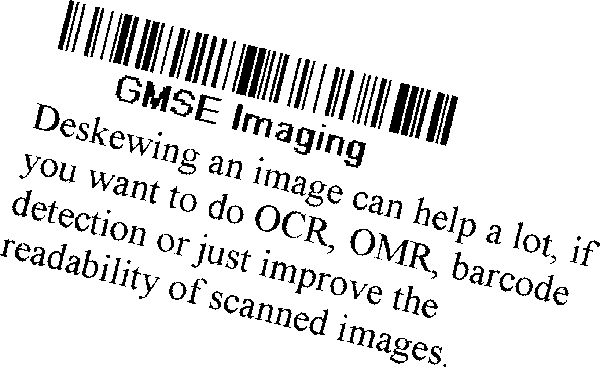
\includegraphics[width=\linewidth]{inclinacion1.png}
			\caption{Imagen antes de aplicar un algoritmo de deskewing }
			\label{fig:minipage1}
	\end{minipage}
	\quad
	\begin{minipage}[b]{0.45\linewidth}
		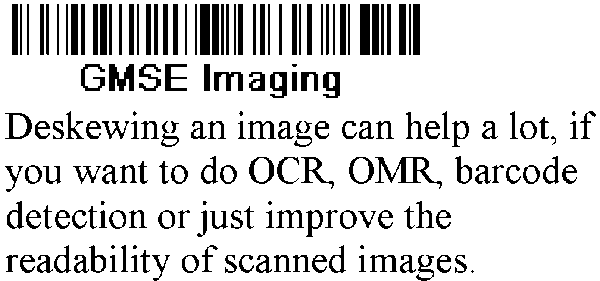
\includegraphics[width=\linewidth]{inclinacion2.png}
		\caption{Imagen después de aplicar un algoritmo de deskewing}
		\label{fig:minipage2}
		\end{minipage}
	\end{figure}

	\item \textbf{Binarización:} Transformar una imagen en color, o en escala de grises a blanco y negro, por ello se la denomina imagen binaria.
	
	\item \textbf{Eliminación de lineas:} Consiste en la eliminación de lineas de texto y cajas en las que el texto pueda estar incrustado (ver figura \ref{fig:lineas}).
	\begin{figure}[ht]
		\centering
		\begin{minipage}[b]{0.45\linewidth}
			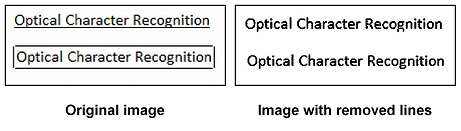
\includegraphics[width=\linewidth]{lineas1.png}
			\caption{Eliminación de lineas en un OCR}
			\label{fig:lineas}
	\end{minipage}
	\end{figure}
	\item \textbf{Zoning:} En esta etapa, el OCR detecta las posiciones de los elementos importantes de la imagen, por ejemplo columnas, párrafos etc..
	\item \textbf{Detección de lineas y palabras:} Se encarga de encontrar las lineas de texto y separarlas por palabras si es necesario.
	\item \textbf{Segmentación:} En muchos textos, los caracteres están divididos en partes, o por el contrario, se tocan entre ellos.
	Por ello es necesario detectar y corregir la posición de cada carácter.
\end{enumerate}

\subsection{Reconocimiento de Caracteres}

Existen dos algoritmos básicos para un OCR.

\subsubsection{Coincidencia de patrones}
Este método consiste en comparar una imagen con un patrón almacenado previamente, para ello se compara pixel por pixel.
Esta técnica funciona mejor con textos mecanografiados, sin embargo la tasa de acierto disminuye  cuando se encuentras con fuentes desconocidas.
\subsubsection{Extracción de características}
Este método utiliza la minería de datos, descompone los caracteres obteniendo sus \textit{características} las cuales son comparadas con la representación abstracta de un carácter cuyo valor ya es conocido, lo que genera una salida de posibles  caracteres candidatos.
Los softwares más modernos utilizan el clasificadores de \textit{vecino más cercano} para elegir el candidato más votado.

El software OCR empleado en este trabajo, Tesseract (ver sección \ref{Tesseract}, emplea un enfoque de dos pasos para el reconocimiento de texto.
Este segundo paso, el cual se denomina reconocimiento de adaptación, permite reconocer los caracteres que no han sido identificados en la primera pasada, utilizando las formas de las letras reconocidas con un grado alto de confianza.

\subsection{Post-Procesado} 
En la ultima fase, se busca aumentar la precisión de el OCR, esto se puede hacer si la salida está limitada por un léxico, por ejemplo las palabras en un idioma,o un léxico de un campo especifico.

La salida de texto se produce en un texto plano, o a un fichero.

\section{Operadores Morfológicos}
La morfología se refiere a un conjunto de operaciones utilizadas para procesar imágenes basándose en formas \cite{OperadoresMorfologicos}. Estas operaciones aplican un elemento estructural (i.e, un cuadrado, una linea, una circunferencia, etc.) sobre una imagen , obteniendo como resultado una imagen de salida del mismo tamaño.
El elemento estructural se compone de una forma y un radio, siendo ambos los parámetros de entrada para el operador. Mediante la modificación de los dos parámetros, se obtendrán diferentes resultados al aplicar el operador.

\imagen{operadorMorfologico}{Operador Morfológico con radio 1 y linea de 45º}
Los operadores funcionan de forma que un pixel p en la imagen de salida se obtendrá a partir de la comparación de ese mismo pixel p en la imagen de entrada con sus vecinos. Los vecinos de p serán precisamente el conjunto pixeles cubiertos por el elemento estructural al tomar como centro del elemento estructural p (ver figura \ref{fig:operadorMorfologico}). La comparación varia en función del tipo de operación estructural aplicada, siendo los tipos mas básicos la erosión, la dilatación.

\section{Erosión y Dilatación}

Los operadores erosión y dilatación se consideran como las operaciones básicas de morfología. Las operaciones son opuestas, en cuanto a que aplicando la erosión se consigue eliminar pixeles en los bordes de la imagen, y aplicando la dilatación se añaden pixeles en los bordes de la imagen.El numero de pixeles añadidos o eliminados dependerá de el elemento estructural y el radio elegidos (ver figura \ref{fig:erodeAndDilate}).

\imagen{erodeAndDilate}{Operaciones de erosión y dilatación con diferentes elementos estructurales}

En una operación de erosión, el valor de un pixel p en la imagen de salida corresponde al mínimo valor en el vecindario de p en la imagen de entrada.

En una operación de dilatación, el valor de un pixel p en la imagen de salida corresponde al máximo valor en el vecindario de p en la imagen de entrada.

\section{Transformada de Hough} \label{Hough}

La transformada de Hough se trata de una técnica que permite detectar figuras que pueden ser expresadas matemáticamente  en imágenes digitales, como por ejemplo rectas, círculos o elipses\cite{wiki:Hough}.

La operación mas simple para la transformada de Hough es la detección de lineas en el espacio de la imagen.
La recta se representa con la ecuación $\mathbf{y= m*x+n}$  y se calcula para cada par de puntos $ \mathbf{\left ( x,y \right )}$ de la imagen.

En el presente trabajo, se ha empleado esta operación para calcular el ángulo de inclinación de una imagen, para poder aplicar un algoritmo de deskewing(ver sección\ref{deskewing}).


\section{Distancia de Levenshtein \label{levenshtein}}
La distancia de Leveshtein nos da el número mínimo de operaciones requeridas para transformar una cadena de texto en otra, las operaciones pueden ser inserción, eliminación o sustitución de un carácter\cite{wiki:Levenshtein}.
Este algoritmo es ampliamente utilizado en operaciones de matching entre cadenas, un ejemplo muy conocido son los correctores ortográficos. 

Matemáticamente , la distancia Levenshtein entre dos cadenas de texto a,b de longitud $\left | a \right |$ y $\left | b \right |$ respectivamente, es dada por:
$
\mathbf{lev}_{a,b}\left ( \left | a \right |,\left | b \right | \right )$
donde:

\begin{center}
\begin{equation}
\mathbf{lev_{a,b}}\left ( i,j \right )\left\{\begin{matrix}
\mathbf{max}\left ( i,j \right ) && if(min\left ( i,j \right ))= 0\\ 
\mathbf{min}\left\{\begin{matrix}
\mathbf{lev_{a,b}}\left ( i-1,j \right )+1\\ 
\mathbf{lev_{a,b}}\left ( i,j-1 \right )+1 & otherwise\\
\mathbf{lev_{a,b}}\left ( i-1,j-1 \right )+1  _{\left (a_{i}\neq b_{j} \right )}
\end{matrix}\right.
\end{matrix}\right.
\end{equation}
\end{center}


En la cual $1_{\left (a_{i}\neq b_{j} \right )}$
es el indicador de función igual a 0 cuando 
$a_{i}= b_{j}$, y $lev_{a,b}\left ( i,j \right )$ es la distancia entre el primer \textit{i} carácter de la primera cadena y el carácter \textit{j} de la segunda cadena.

Por ejemplo la distancia Levenshtein entre casa y calle es de 3 dado que se necesitan 3 operaciones  para cambiar una por la otra.
\begin{enumerate}
	\item casa $\rightarrow $ cala (sustitución de 's' por 'l')
	\item cala $\rightarrow $ calla (inserción de 'l')
	\item calla $\rightarrow $ calle (sustitución de 'a' por 'e')
\end{enumerate}

En el presente trabajo ha permitido corregir los errores cometidos por Tessertact al traducir una imagen a texto, todo ello apoyándose en un fichero de texto que se emplea a modo de diccionario.

\section{Tipos de tiques}

Un tique es un papel que se da a un cliente en el que se refleja el importe que ha pagado por una compra o un servicio, por el cual el usuario tiene derecho a reclamar por el articulo\cite{tique}.

Estos tiques están formados por un desglose de los artículos adquiridos, de los cuales se tiene el conocimiento de la cantidad y el  precio. Esta información se muestra en líneas de texto , que denominaremos a partir de ahora líneas de producto.

Para la realización de este trabajo se ha realizado una fase de clasificación de tiques para determinar si es posible emplearlos para la detección de sus lineas.
El problema encontrado a la hora de analizar estos, es la gran variedad que podemos encontrarnos a la hora de realizar la extracción de sus lineas de producto.
\begin{figure}[ht]
		\centering
		\begin{minipage}[b]{0.45\linewidth}
			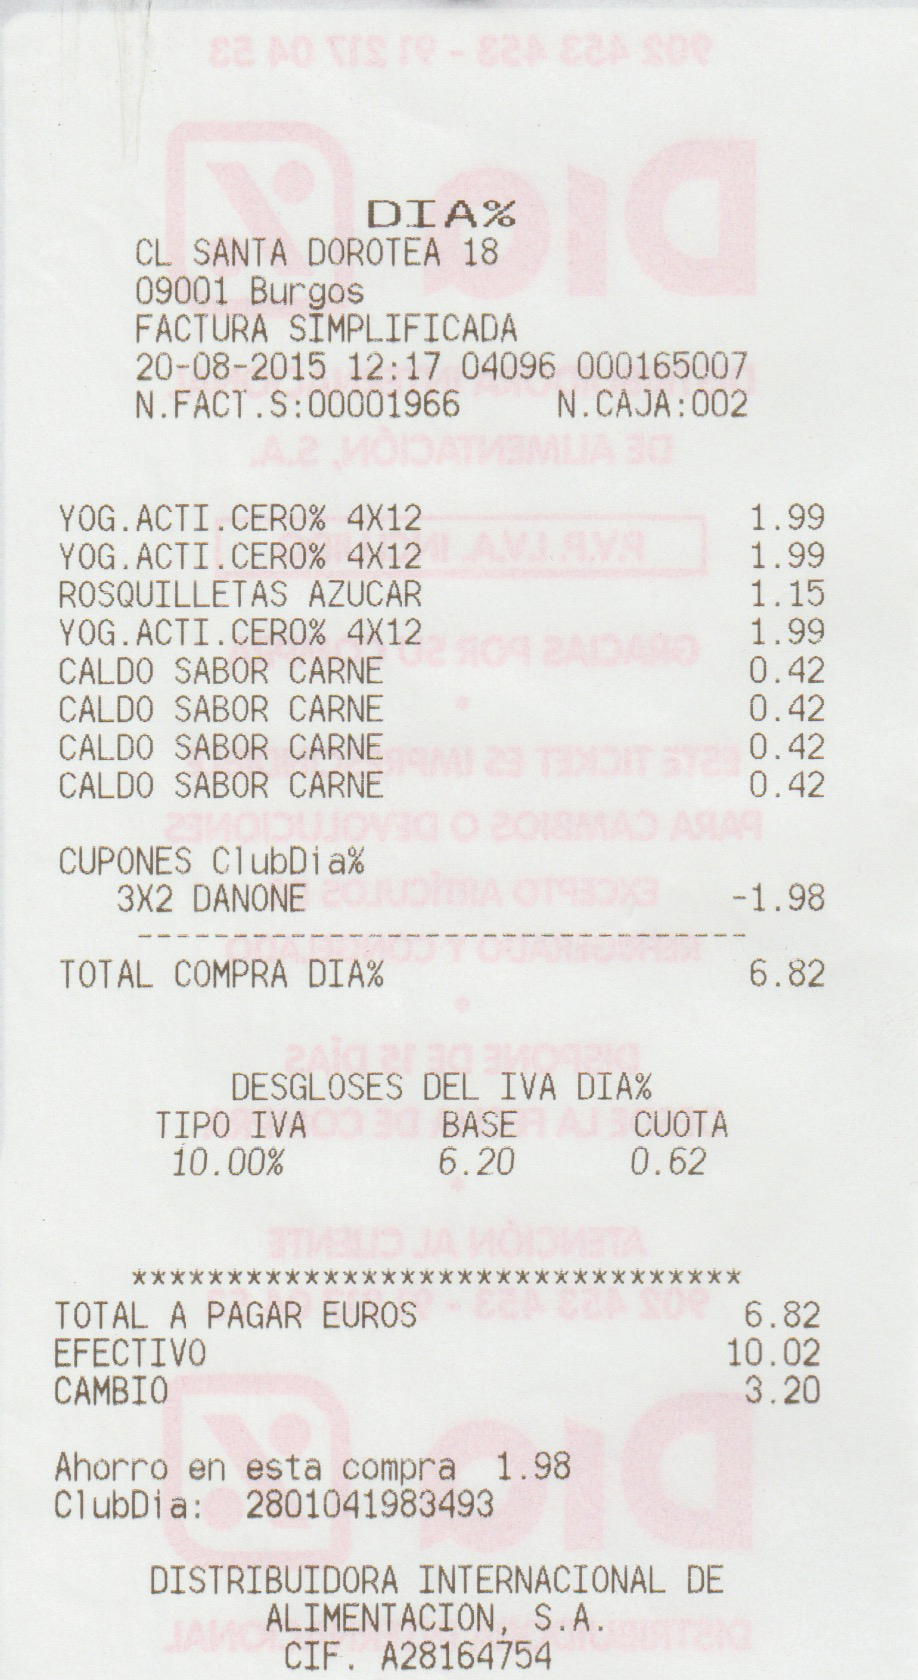
\includegraphics[width=\linewidth]{tique1.jpg}
			\caption{Tique con 2 columnas}
			\label{fig:minipage1}
	\end{minipage}
	\quad
	\begin{minipage}[b]{0.45\linewidth}
		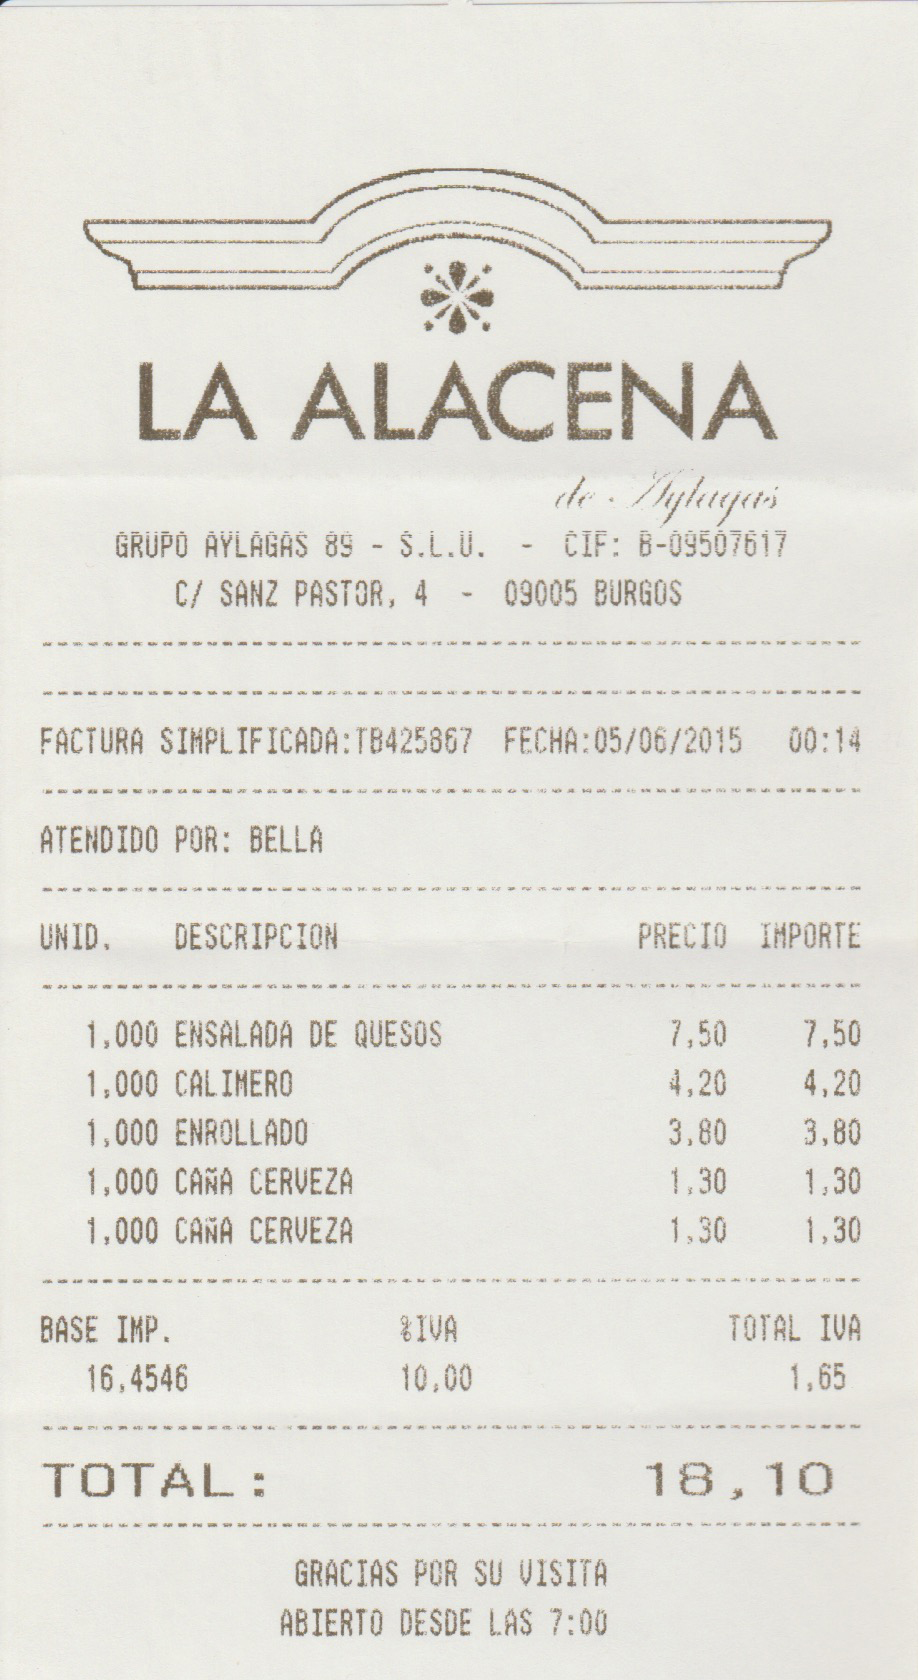
\includegraphics[width=\linewidth]{tique2.jpg}
		\caption{Tique con 4 columnas}
		\label{fig:minipage2}
		\end{minipage}
		\quad
		\begin{minipage}[b]{0.45\linewidth}
			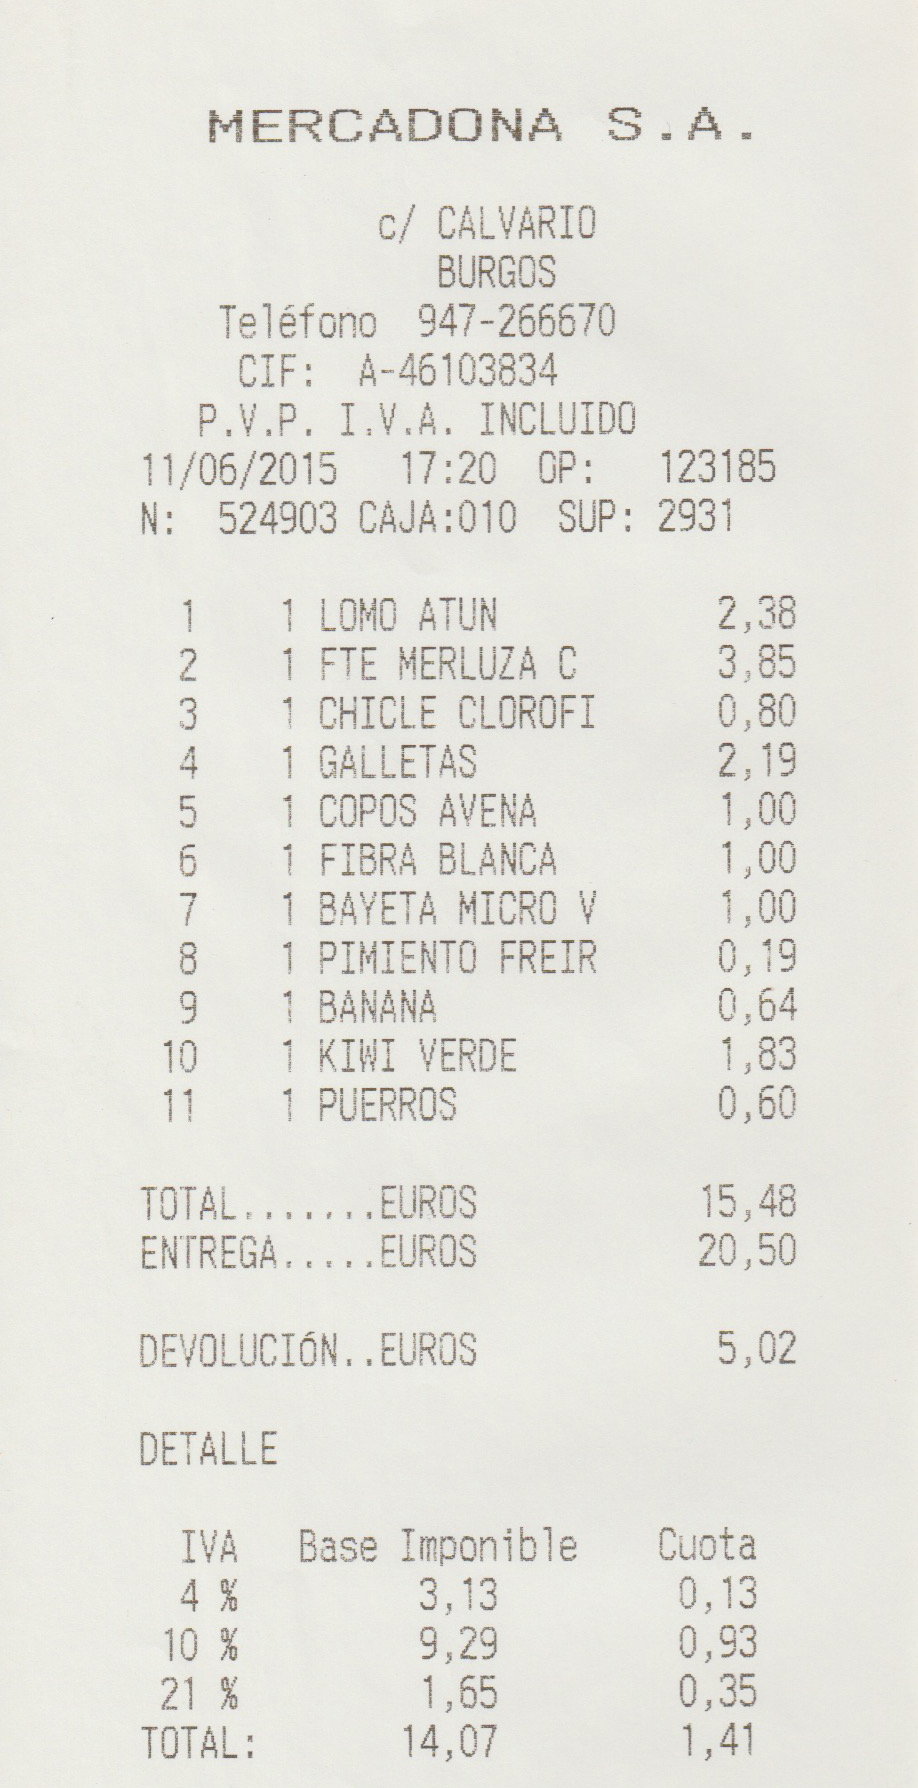
\includegraphics[width=\linewidth]{tique3.jpg}
			\caption{Tique con 4 columnas}
			\label{fig:minipage3}
	\end{minipage}
	\quad
	\begin{minipage}[b]{0.45\linewidth}
		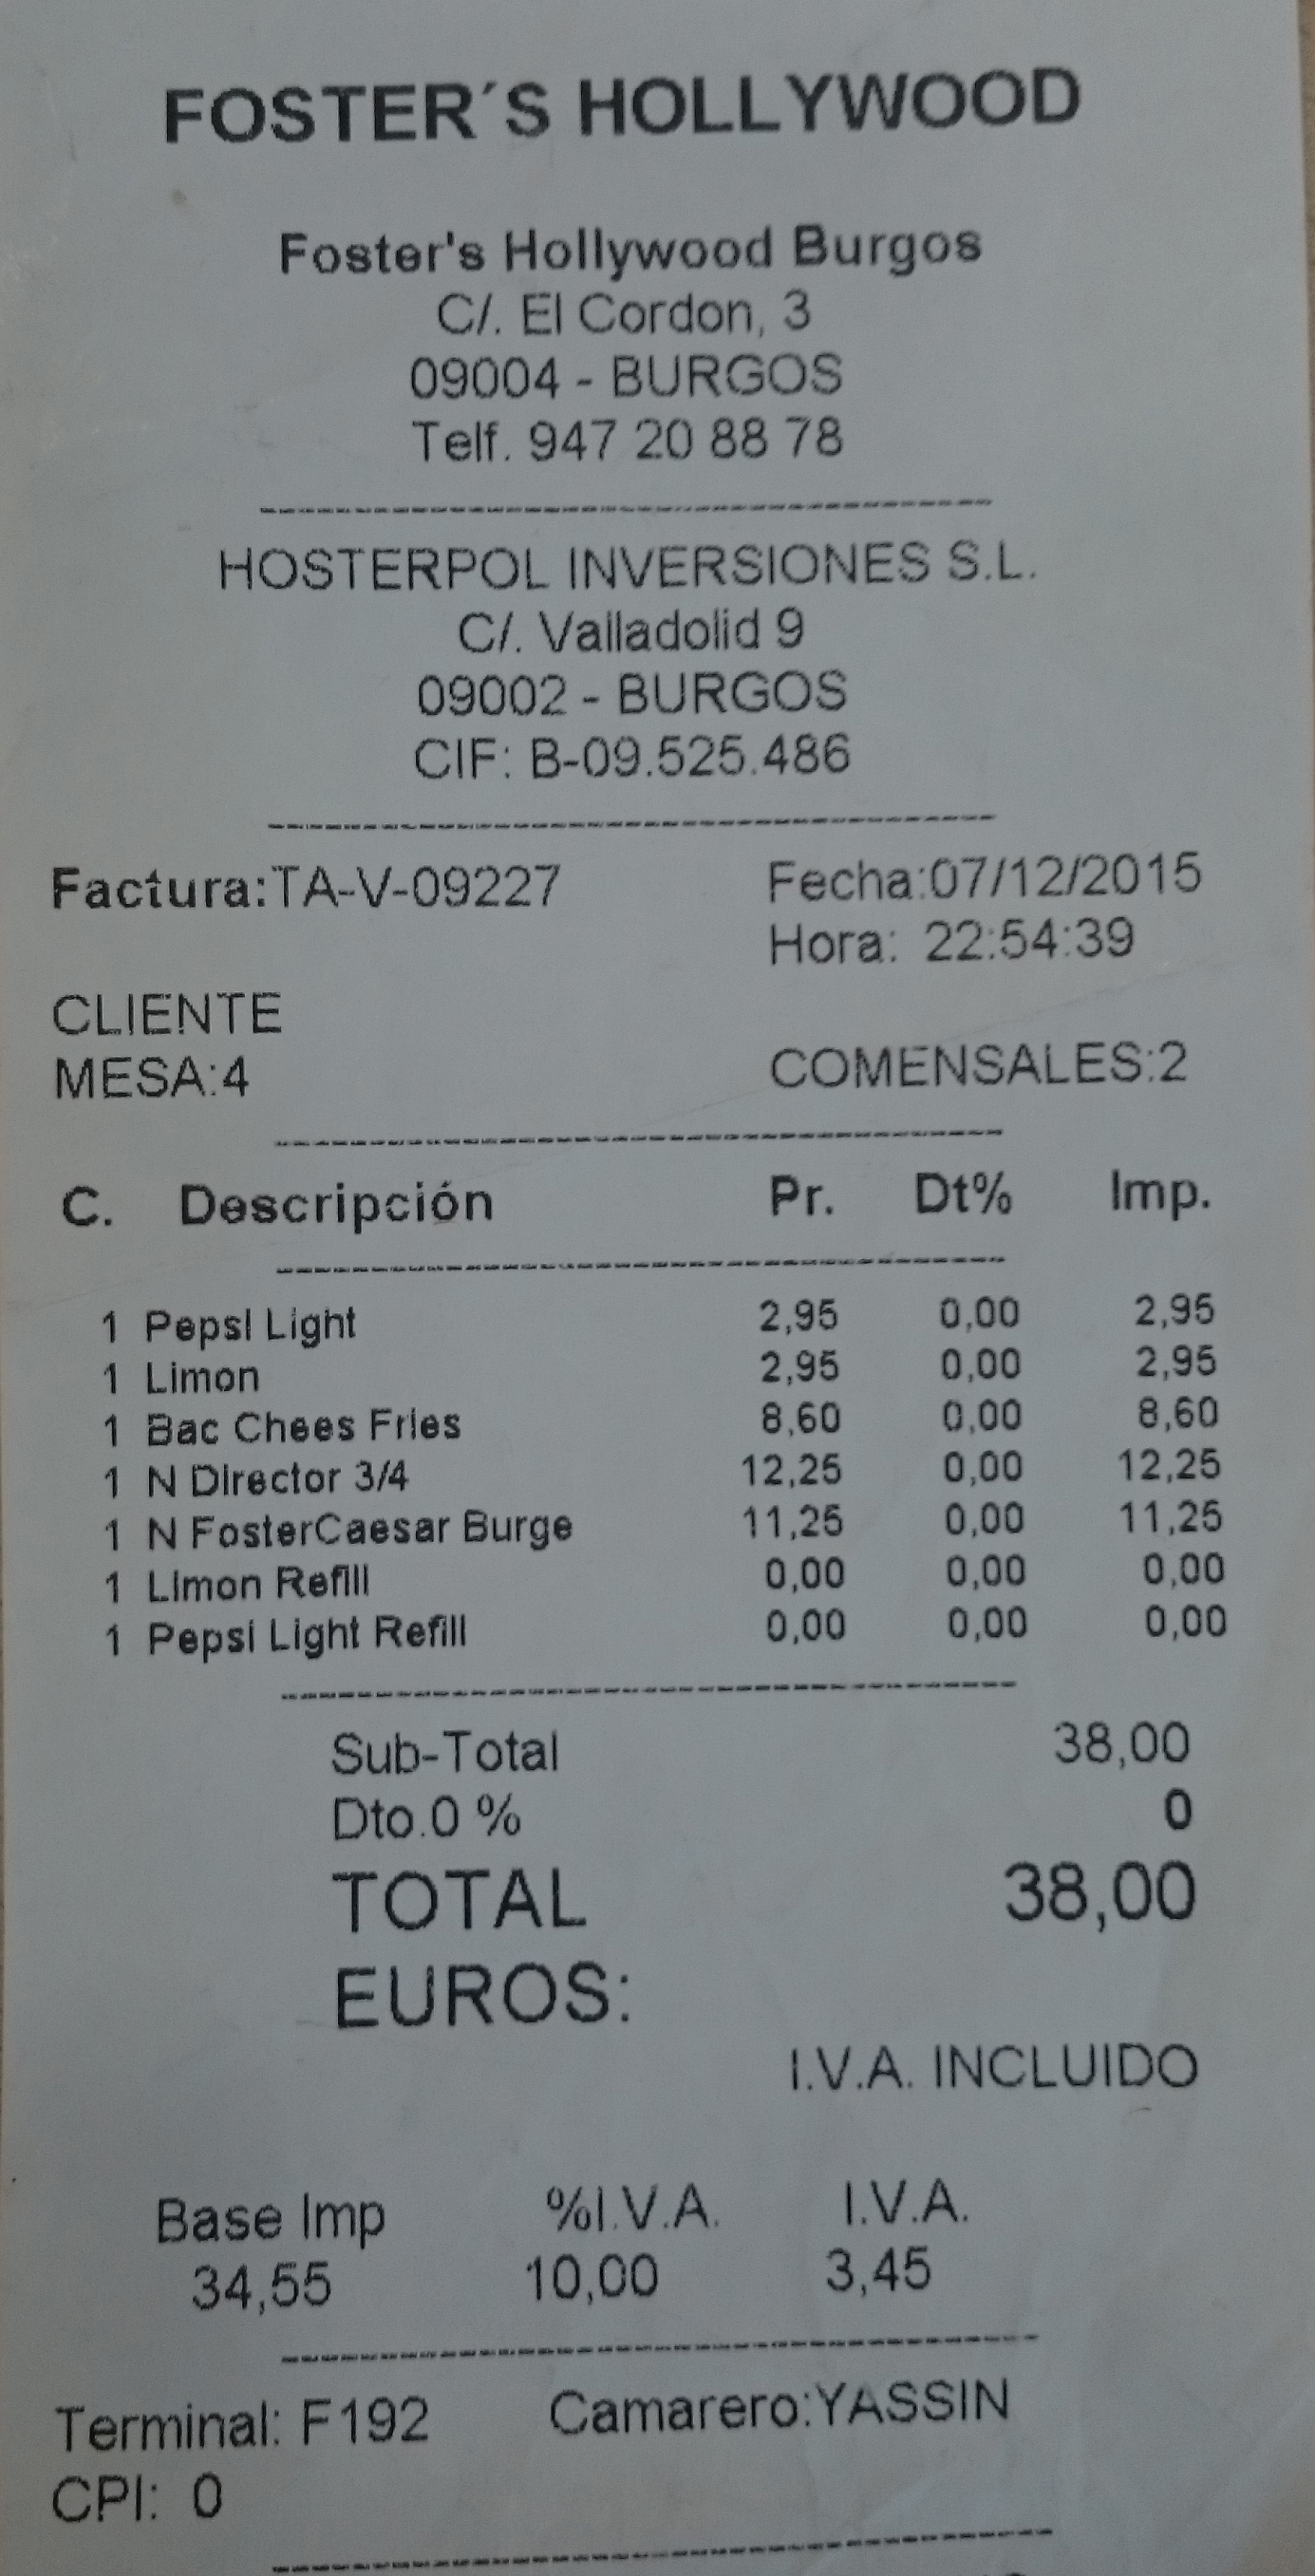
\includegraphics[width=\linewidth]{tique4.jpg}
		\caption{Tique con 5 columnas}
		\label{fig:minipage4}
		\end{minipage}
\end{figure}

\cleardoublepage

Podemos ver como en cada tique las columnas en las que se distribuye la información varía de uno a otro, sin embargo, en los muchos tiques que siguen una distribución de 4 columnas (ver figura \ref{fig:minipage2}) estas se distribuyen de la siguiente manera:
\begin{itemize}
	\item Unidades.
	\item Descripción.
	\item Precio.
	\item Importe.
\end{itemize}

Por lo que es posible abarcar un numero elevado de tiques, ya que este modelo, se emplea principalmente en establecimientos de hostelería y restauración.


\section{Modelo Cliente-Servidor}

La arquitectura cliente-servidor es un modelo de aplicación distribuida en cual las que las tareas se reparten entre los proveedores de servicios o servidores, y los demandantes denominados clientes \cite{wiki:Cliente-servidor}.

El cliente realiza las peticiones a un programa, que se encuentra en el servidor, y este le devuelve una respuesta de vuelta al cliente (ver figura \ref{fig:client_server}), por ello toda la gestión de la información y responsabilidad se encuentra en el servidor.

\imagen{client_server}{Peticion-Respuesta de un cliente a un servidor}

Las ventajas de este tipo de arquitectura son: 
\begin{itemize}
	\item \textbf{Uso de recursos:} El uso de un servidor permite a los clientes el uso de los recursos de este, lo que facilita la ejecución de tareas mas costosas en un tiempo menor.
	\item \textbf{Escalabilidad:} Es posible añadir nuevos clientes en cualquier momento.
	\item \textbf{Facilidad de mantenimiento:} Dado que el cliente y el servidor son maquinas distintas, es posible realizar cambios en este ultimo sin que el cliente se vea afectado, lo que permite añadir nuevas funcionalidades sin la necesidad de cambiar los clientes.
\end{itemize}

Sin embargo, este modelo presenta dos desventajas muy claras:
\begin{itemize}
	\item \textbf{Necesidad de una conexión:} Es necesario mantener un canal de conexión entre el cliente y el servidor.
	\item \textbf{Disponibilidad:} El servidor debe estar disponible en todo momento, dado que el resto de maquinas depende de el.
\end{itemize}

La mayoría de los servicios que se proporcionan en la actualizad utilizan esta estructura.


\section{Api-Rest}
Representational State Transfer o Rest es una arquitectura software apoyada en un modelo cliente-servidor y el protocolo HTTP \cite{wiki:rest}.

Este modelo se utiliza para definir a un sistema que utiliza el protocolo HTTP para realizar llamadas al servidor con una serie de parámetros, los cuales son los datos  a interpretar por el servidor, una vez procesados se genera una respuesta que se devuelve al cliente, generalmente en formato XML o JSON.

En el presente trabajo, se ha construido un servicio REST que recibe como parámetro una imagen de un tique y devolver los productos que se han encontrado en este, empaquetados en un JSON.

\section{JSON}

JSON es un acronimo para JavaScript Objet Notation, es un estandar de texto plano, empleado para el intercambio de datos. La ventaja de este formato es que es independiente del lenguaje de programación en los que las maquinas están programadas, cada lenguaje tiene su propia librería para codificar y descodificar cadenas JSON \cite{json}.

La formación de un objeto JSON se realiza con pares atributo-valor que deben estar encerrados entre llaves y separados por comas, las cuales definen el principio y el fin del objeto.

Un ejemplo: \textit{$\{
"nombre":"Roberto",
"edad":23
\}$}

\capitulo{4}{Técnicas y herramientas}

En este apartado se describen las metodologías usadas y las herramientas de desarrollo que se han utilizado en el presente trabajo.

\section{Metodologia ágil Scrum \label{scrum}}
Scrum es una metodología de desarrollo ágil, la cual, está basada en iteraciones llamadas sprints. Cada iteración termina con una pieza de software que añade una nueva funcionalidad o mejora las ya existentes. Esta iteraciones suelen durar de 2 a 4 semanas\cite{scrum}.
Como elementos clave del Scrum podemos encontrar:
\begin{itemize}
\item Entregas periódicas de de funcionalidades del producto que se está desarrollando
\item Se desarrolla una serie de reuniones de equipo para determinar las tareas que se van a realizar en cada iteración.
\end{itemize}

Para el desarrollo del presente trabajo, las iteraciones se han desarrollado con un periodo de una a dos semana.

\section{Herramientas}
En esta sección aparecen cada una de las herramientas utilizadas para la realización del proyecto.
Se han dividido en categorías en función de su uso:
\begin{itemize}
	\item \textbf{Herramientas de desarrollo}
	\item \textbf{Herramientas de gestión}
	\item \textbf{Herramientas de documentación}
	\item \textbf{Herramientas externas}
\end{itemize}

\subsection{Herramientas de desarrollo:}
\subsubsection{NetBeans}
Como entorno de desarrollo de la aplicación por parte del servidor se ha utilizado NetBeans. Se ha decidido trabajar con esta herramienta por su incorporación de el servidor de Glassfish.
NetBeans es un proyecto open source fundado por Sun MicroSystem. El IDE soporta todos los tipos de aplicación Java(J2SE,web y aplicaciones móviles).

Página web de la herramienta: \url{https://netbeans.org/}

\subsubsection{Android Studio}
Android Studio es un entorno de desarrollo para la plataforma de Android, basado bajo el software de IntelliJ IDEA y desarrollado por Google. Como principales características soporta refactorizaciones especificas para Android, y plantillas para la creación de diseños.

Página web de la herramienta: \url{http://developer.android.com/intl/es/sdk/index.html}
\subsection{Herramientas de gestión:}

\subsubsection{Git}
Git es un software de control de versiones diseñado por Linus Torvalds, pensado para el mantenimiento de versiones de aplicaciones cuando estas tienen un volumen elevado de archivos con código fuente.

Página web de la herramienta: \url{https://git-scm.com/}

\subsubsection{Bitbucket} 
Bitbucket es una web de alojamiento de proyectos basados en Git o Mercurial. Esta herramienta nos permite tener un control de versiones de nuestros proyecto, como principal ventaja es la privacidad de estos de forma gratuita.

Página web de la herramienta: \url{https://bitbucket.org}

\subsubsection{SourceTree}
SourceTree es una aplicación de escritorio para MacOS y Windows que permite el control de proyectos Git o Mercurial.
Como característica principal es su interfaz clara y de fácil manejo permitiendo de un vistazo ver los commits realizados, los branches, etc..
Es gratuita, pero necesario realizar un registro para su funcionamiento.

Página web de la herramienta: \url{https://www.sourcetreeapp.com/}

\subsection{Version One}
VersionOne es una aplicación web que permite gestionar proyectos.
En ella se utiliza Scrum(ver sección \ref{scrum}) para gestionar estos, permitiendo crear sprints y tareas asociadas. Permite ver el seguimiento mediante una representación de gráficos, llamados Burndown.

Página web de la herramienta: \url{http://www.versionone.com/}

\subsection{Herramientas de documentación:}

\subsubsection{\TeX{}Maker}
TextMaker es un editor Latex multiplataforma.
Permite la creación de documentos en PDF permitiendo la rápida localización de cada comando de Latex.

Página web de la herramienta: \url{http://www.xm1math.net/texmaker/}
	
\subsection{Herramientas externas:}
Estas herramientas se han empleado para la simplificación del desarrollo del presente proyecto, dado que sin ellas seria prácticamente imposible llevarlo a cabo.

\subsubsection{Tesseract} \label{Tesseract}
Teserract es un motor OCR desarrollado actualmente por Google bajo licencia Apache.
Esta considerado uno de los mejores motores en cuanto precisión, multiplataforma y con una versión para Android, sin embargo el funcionamiento y precisión de esta versión esta lejos de una versión más madura como las de escritorio, por ello se ha decidido incorporar esta funcionalidad en la parte del servidor.

Página web de la herramienta:
 
\url{https://github.com/tesseract-ocr/tesseract}

\subsubsection{OpenCV}
OpenCv es una librería de procesamiento de imágenes. Esta librería contiene una gran cantidad de algoritmos para el procesado de imágenes y una comunidad de usuarios muy elevada. La ventaja de OpenCV es su versatilidad a la hora de emplearse en diferentes plataformas y S.O. Utiliza una licencia BSD

Página web de la herramienta: \url{http://opencv.org/}

\subsubsection{GlassFish}
GlassFish es un servidor de aplicaciones java desarrollado por Oracle.
Existen 2 versiones una de código libre y otra versión comercial, en este proyecto se ha usado la versión gratuita, bajo las licencias CDDL y la GNU GPL.

Página web de la herramienta: \url{https://glassfish.java.net/}

\subsubsection{Jersey}
Jersey es un framework que permite simplificar la creación de un WebService.
Esta herramienta se basa en el la api \textit{JAX-RS (Java API for RESTful Web Services)} \cite{wiki:JAX-RS} que proporciona soporte para la creación de servicios web RESTFul, a la cual, jersey añade nuevas características y utilidades para simplificar el proceso de desarrollo de una API REST.
La principal ventaja de jersey es que incluye compatibilidad con GlassFish.

Página web de la herramienta: \url{https://jersey.java.net}

\subsubsection{SQLite}
SQLite es un motor de base de datos relacional, como principal característica destaca por su pequeño tamaño del fichero utilizado para contener los datos, por ello es perfecto para dispositivos de memoria limitada como smartphones o werables.

Página web de la herramienta: \url{https://www.sqlite.org}

 
 \subsubsection{OrmLite}
 OrmLite es un \textit{Object Relational Mapping (ORM)} que permite la conversión de nuestros objetos en datos persistentes nuestro sistema de persistencia, en este caso una BD en Sqlite. Soporta funionamiento en la plataforma de android y sus principales ventajas son:
 	\begin{itemize}
 		\item Configuración de los objetos  mediante anotaciones.
 		\item Abstracción de los objetos mediante el patrón DAO.
 		\item Construcción de consultas de forma sencilla.
 	\end{itemize}
En este proyecto, se ha empleado para la persistencia de los tiques en la base de daros del smartphone.

Página web de la herramienta: \url{http://ormlite.com/}

\subsubsection{SimpleCropView}

SimpleCropView es una biblioteca para el recortado de  imágenes en Android.
Esta biblioteca simplifica el código y proporciona una interfaz de usuario fácil de personalizar.

Página web de la herramienta: \url{https://android-arsenal.com/details/1/2366} 

\begin{table}[htb]
\rowcolors {2}{gray!35}{}
\centering
\begin{tabular}{l c c c c}
\toprule
    Herramienta    & Tipo de Licencia          & Coste \\
    \otoprule
Net Beans      &            -                & 0\euro       \\
Android Studio & Apache License 2.0        & 0\euro      \\
Bitbucket      & -                         & 0 \euro     \\
SourceTree     & -                         & 0 \euro     \\
TexMaker       & GPL License               & 0 \euro    \\
Tesseract      & Apache License 2.0        & 0 \euro      \\
OpenCv         & BSD License               & 0 \euro      \\
GlassFish Free & CDDL y GPL License        & 0 \euro      \\
Jersey         & CDDL y GPL License        & 0 \euro      \\
SQLite         & -                         & 0\euro    \\
OrmLite        & Open source license (ISC) & 0 \euro     \\
SimpleCropView & Apache License 2.0        & 0 \euro   \\
\bottomrule 
\end{tabular}
\label{tabla:herramientas}
\caption{Tabla de herramientas}
\end{table}

\capitulo{5}{Aspectos relevantes del desarrollo del proyecto}

\section{Desarrollo de la idea}

El proyecto inicial surgió a partir de un problema a la hora de repartir  el coste de un tique entre varios usuarios los cuales debían pagar el importe correspondiente por los artículos consumidos por cada uno, la idea era calcular esto de forma automática a partir de una aplicación en la que cada cliente introdujera el importe pagado y los artículos consumidos, los cuales se extraerían a partir de una imagen.

Esta idea se cambio por la siguiente propuesta, llevar a cabo una aplicación de gestión de gastos a partir de la cual, el usuario introduce una imagen de los productos consumidos y estos son almacenados de forma que, el usuario pueda consultar en cualquier momento en que se ha gastado su dinero.

\section{Tesseract como Libreria OCR \label{precisionTesseract}}

Para poder desarrollar el presente trabajo, se realizó una búsqueda preliminar de como poder llevar a cabo la extracción de los productos a partir de una imagen digital, para ello fue necesario la búsqueda de un OCR (\ref{ocr}) para poder realizar la  extracción del texto.
La herramienta propuesta por el tutor fue Tesseract, la cual permitía la obtención del texto a partir de un fichero de imagen, de forma gratuita y con una exactitud aceptable.

Se instaló y probó Tesseract en un entorno Linux, y se realizaron las siguientes pruebas a las imágenes \ref{fig:original1},\ref{fig:recortada1},\ref{fig:original2} y\ref{fig:recortada2}

\begin{itemize}
	\item Sin ninguna configuración con diccionario de caracteres Ingleses.
	\item Configuración en bloque con diccionario de caracteres Ingleses.
	\item Configuración en linea con diccionario de caracteres Ingleses.
	
	\item Configuración en palabra con diccionario de caracteres Ingleses.
	
	\item Sin ninguna configuración con diccionario de caracteres Español.
	\item Configuración en bloque con diccionario de caracteres Español.
	\item Configuración en linea con diccionario de caracteres Español.

\item Configuración en palabra con diccionario de caracteres Español.

\end{itemize}

\begin{figure}[ht]
		\centering
		\begin{minipage}[b]{0.45\linewidth}
			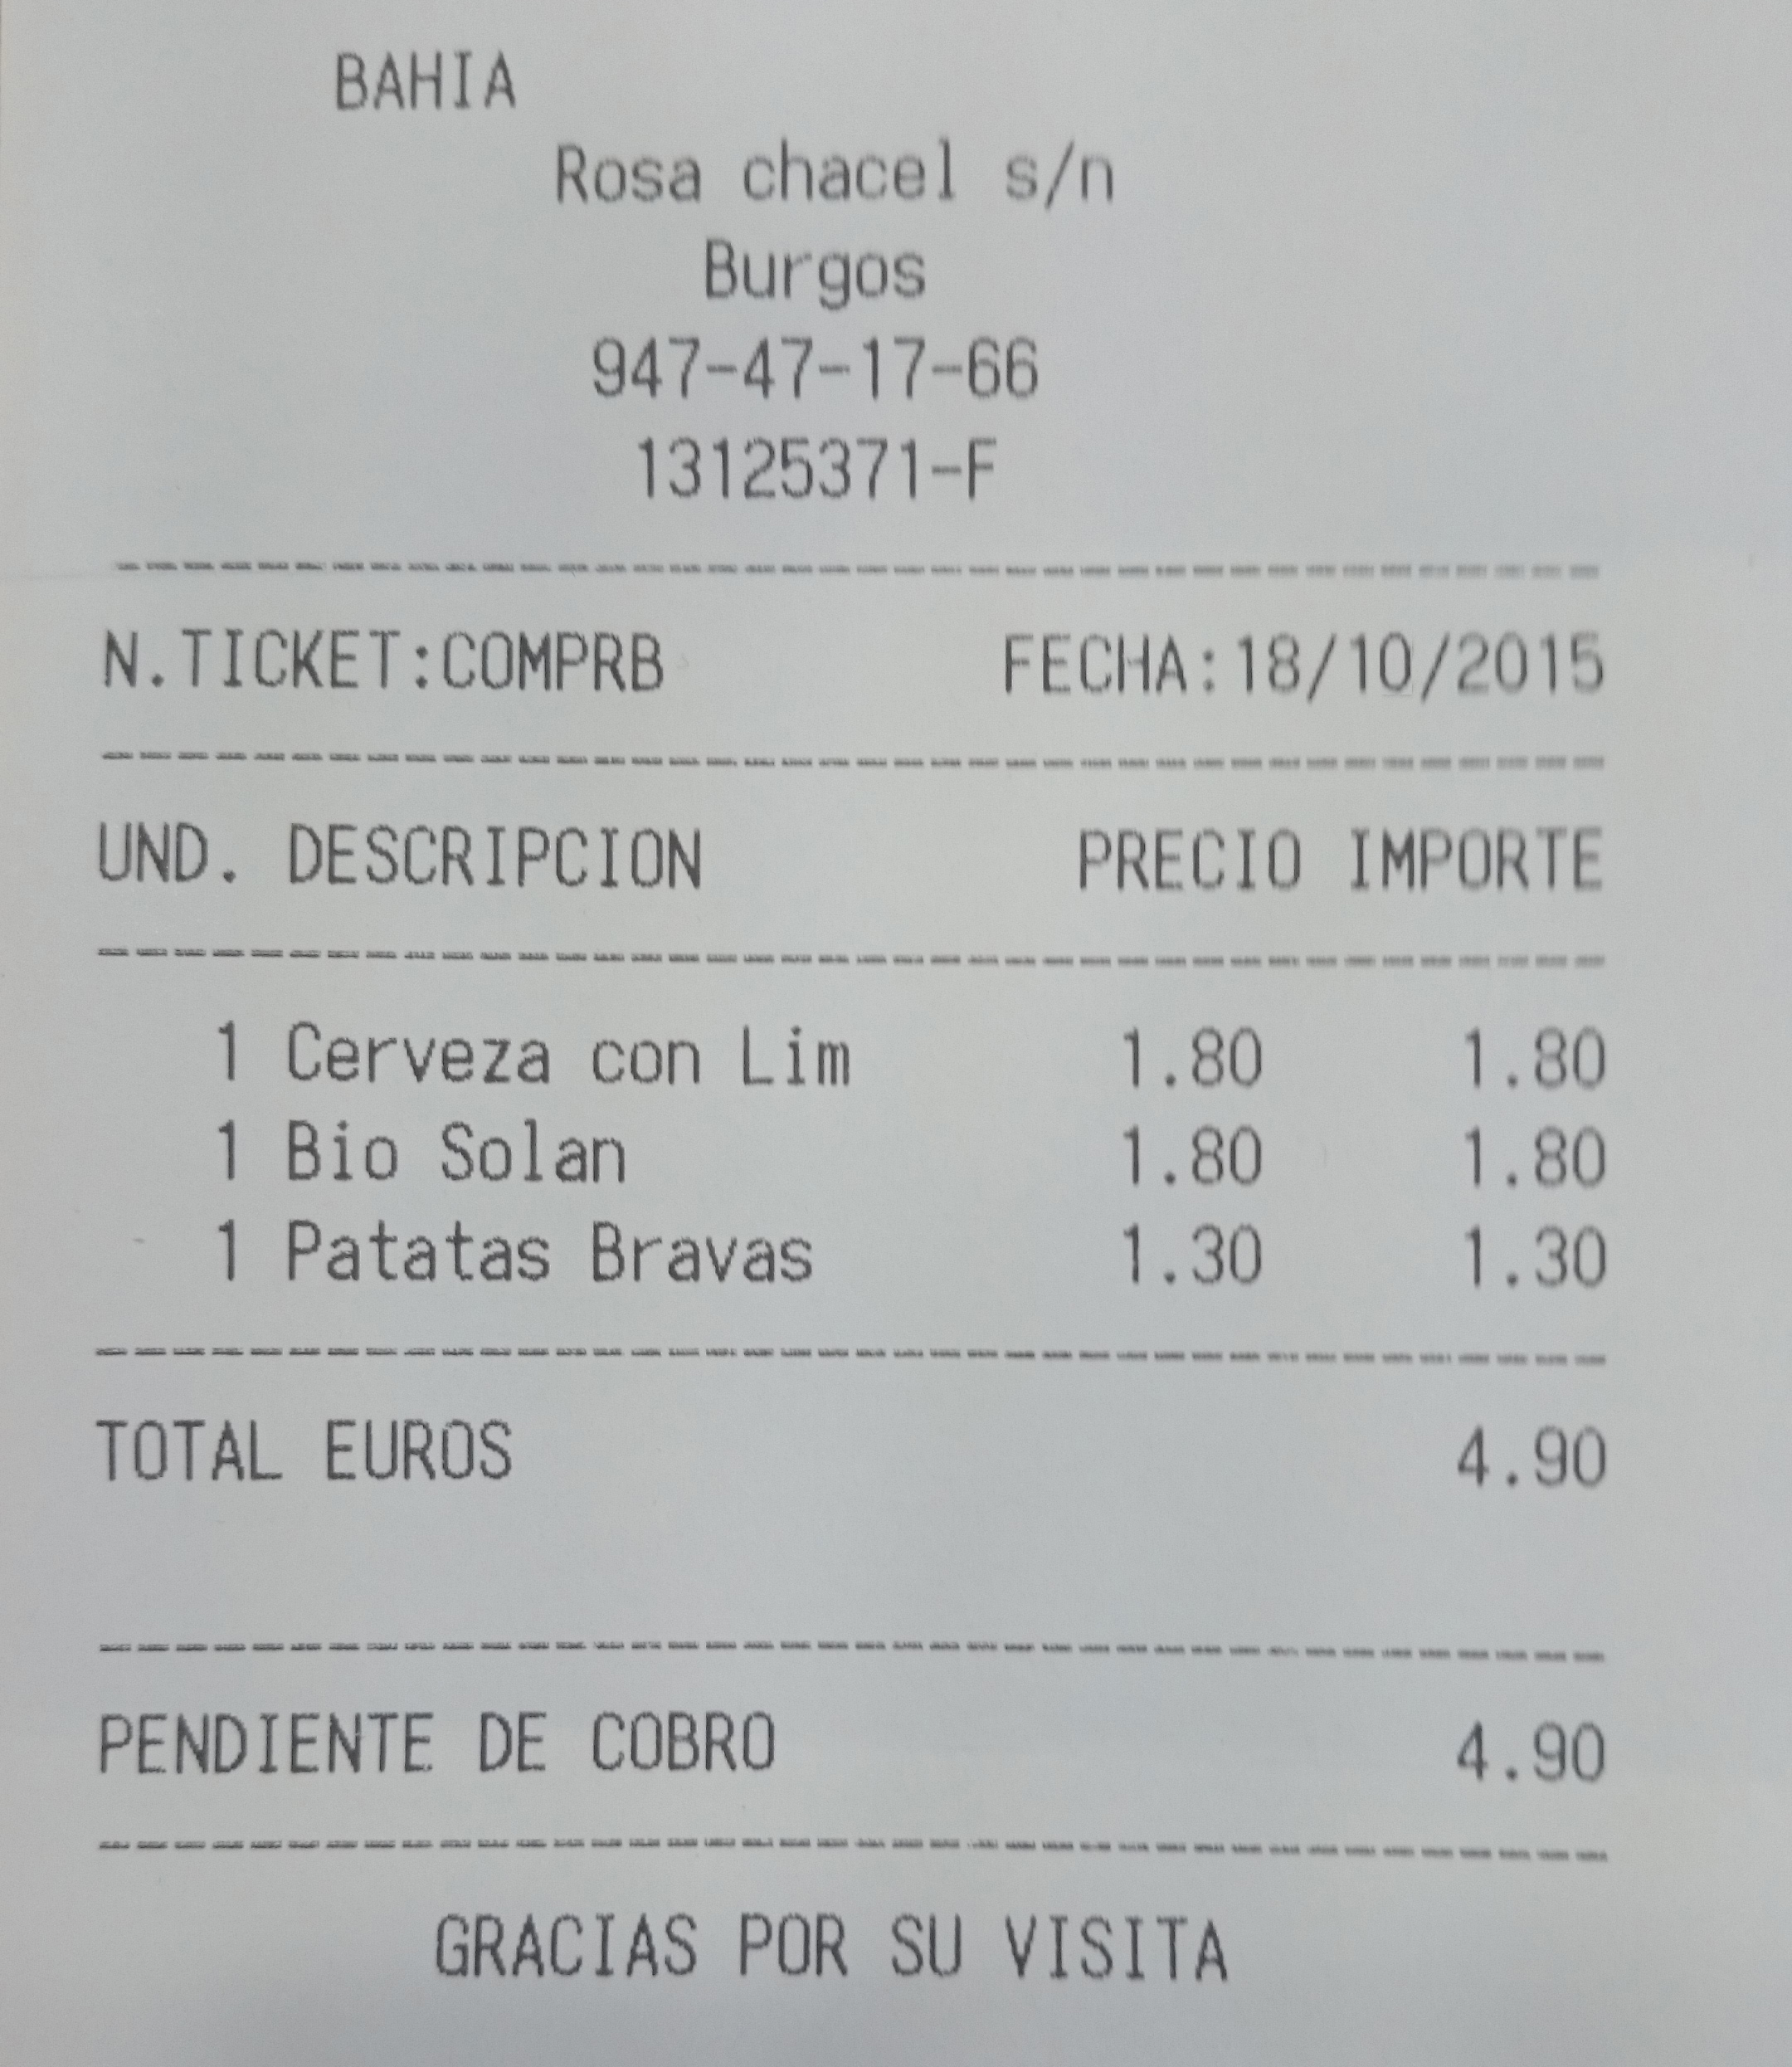
\includegraphics[width=\linewidth]{Original1.jpg}
			\caption{Imagen Original nº 1}
			\label{fig:original1}
	\end{minipage}
	\quad
	\begin{minipage}[b]{0.45\linewidth}
		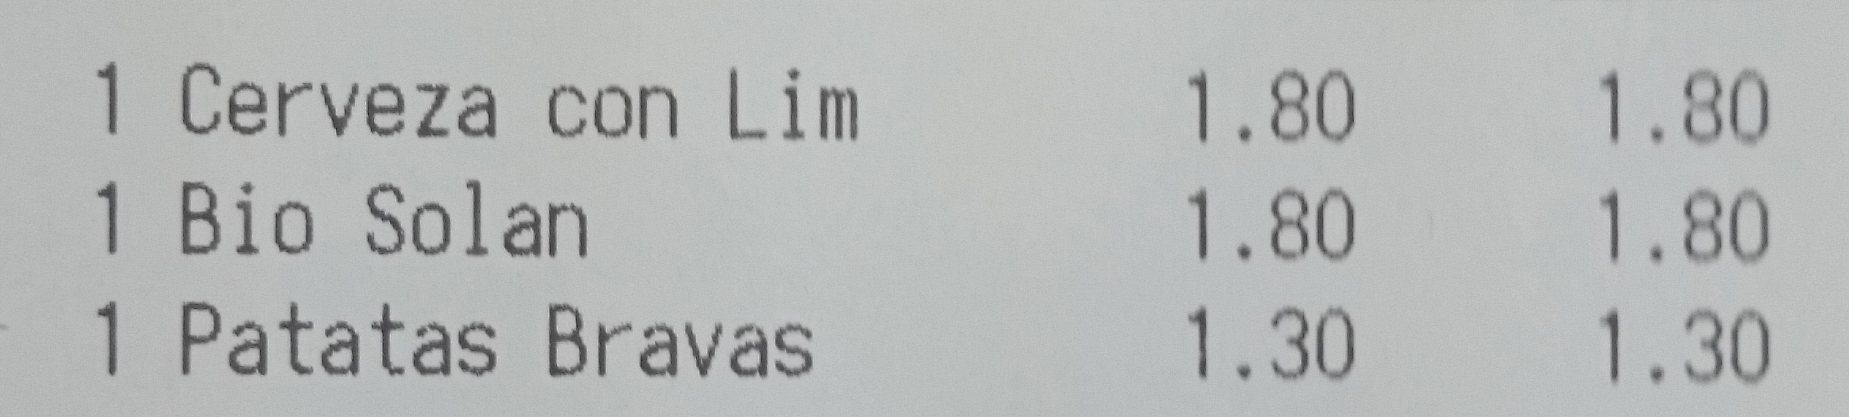
\includegraphics[width=\linewidth]{Recortada1.jpg}
		\caption{Recorte de la imagen original nº 1}
		\label{fig:recortada1}
		\end{minipage}
		\begin{minipage}[b]{0.45\linewidth}
			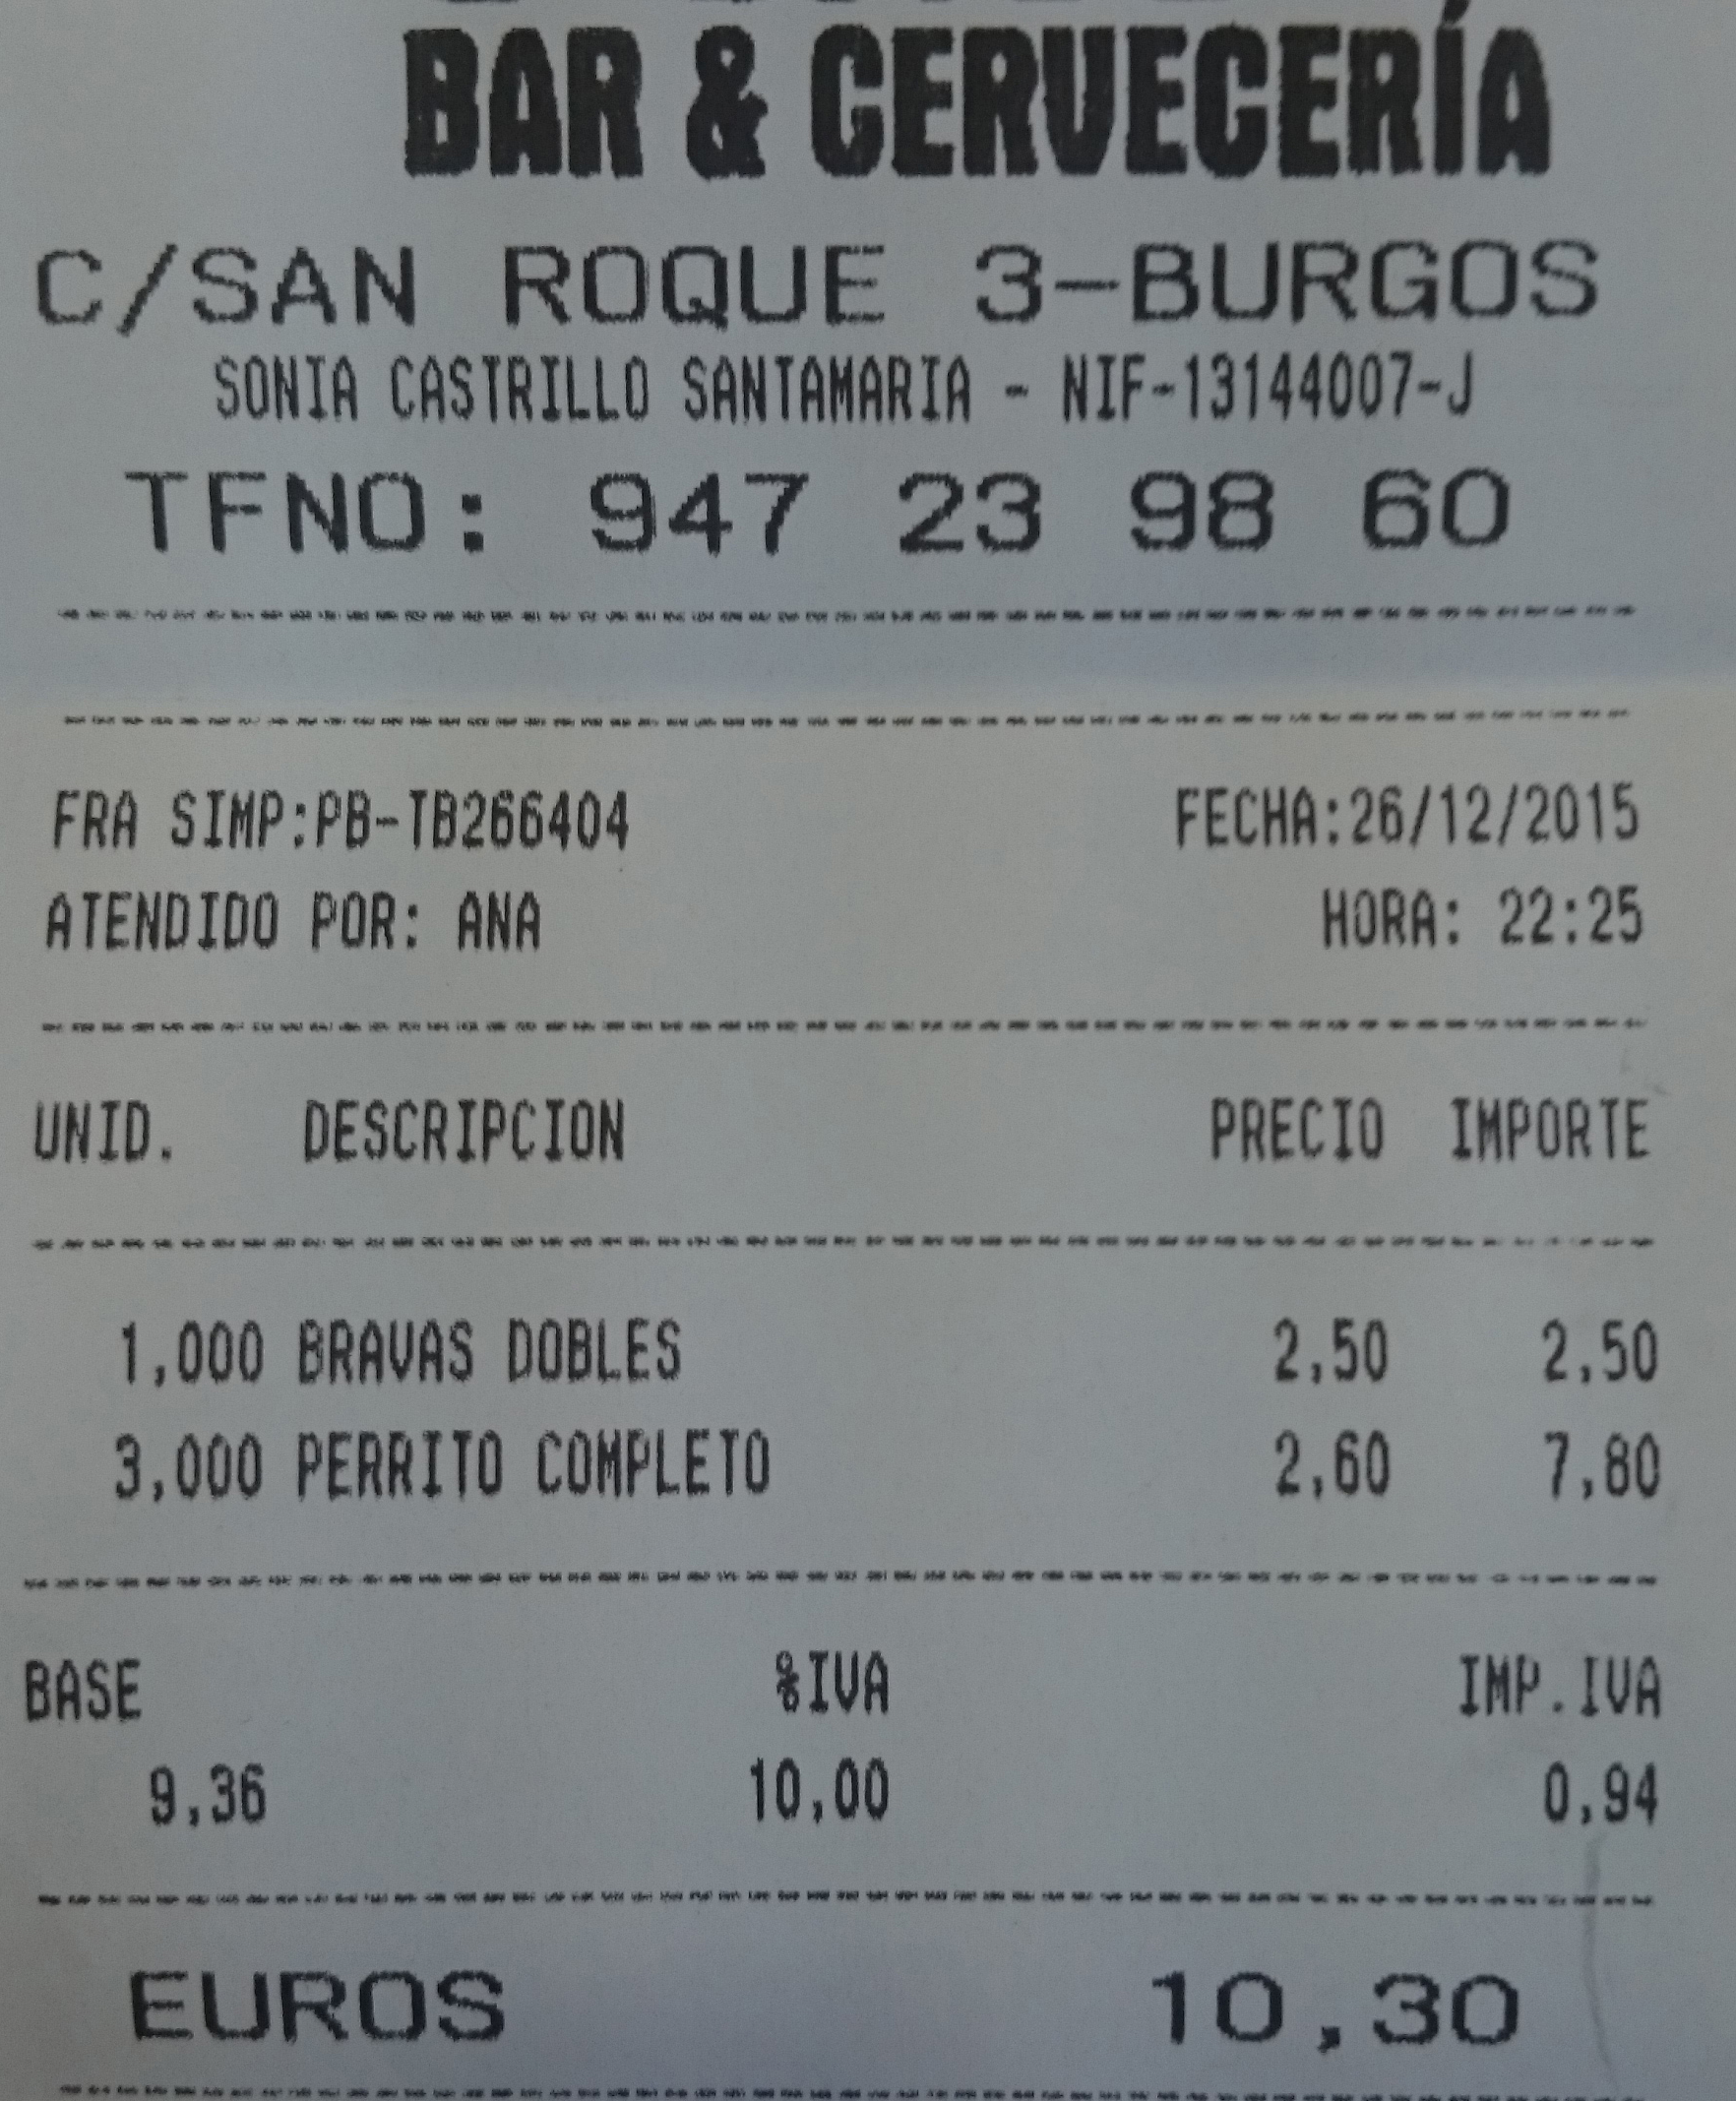
\includegraphics[width=\linewidth]{Original2.jpg}
			\caption{Imagen Original nº 2}
			\label{fig:original2}
	\end{minipage}
	\quad
	\begin{minipage}[b]{0.45\linewidth}
		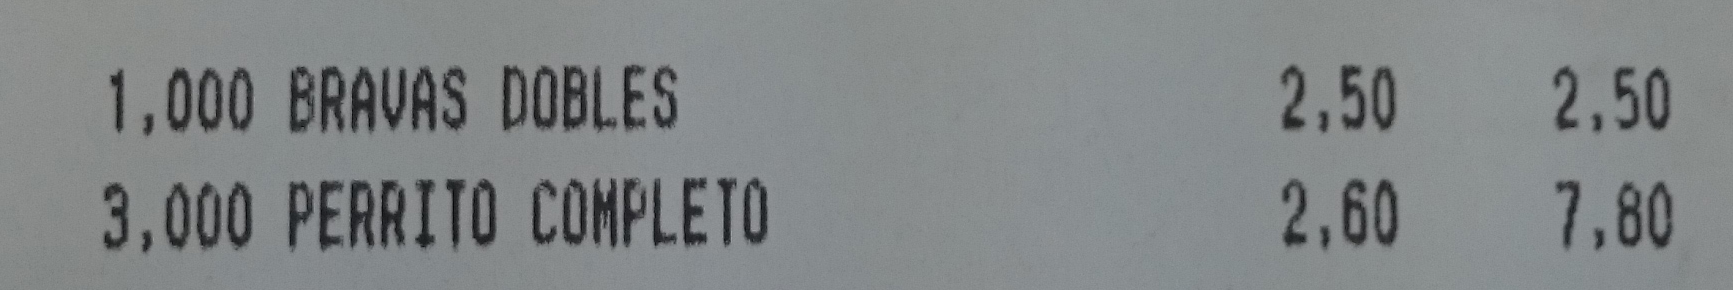
\includegraphics[width=\linewidth]{Recortada2.jpg}
		\caption{Recorte de la imagen original nº 2}
		\label{fig:recortada2}
		\end{minipage}
	\end{figure}
	


\clearpage

Estas pruebas han sido resumidas según el porcentaje de acierto (caracteres acertados / número total de caracteres) en las tablas \ref{tesseractingles} y \ref{tesseractespa}


\begin{table}[ht]
\rowcolors {2}{gray!35}{}
\center
\begin{tabular}{l c c c c}
\toprule
    Imagen    & Normal        & En bloque & En linea & Palabra\\
    \otoprule
Imagen 1     &  0\%   &  0\%     & 0\%   &  0\%\\
Recortada 1  &    61\%&   100\%   & 0\%  & 0\%\\
Imagen 2     &     0\%    &    0\%   &  0\%  &  0\%\\
Recortada 2      &    81\%&   81\%   & 0\%  & 0\%\\
\bottomrule 
\end{tabular}
\label{tesseractingles}
\caption{Pruebas precision Tesseract diccionario Inglés}
\end{table}

\begin{table}[ht]
\rowcolors {2}{gray!35}{}
\center
\begin{tabular}{l c c c c}
\toprule
    Imagen    & Normal        & En bloque & En linea & Palabra\\
    \otoprule
Imagen 1     &  0\%   &  0\%     & 0\%   &  0\%\\
Recortada 1  &    61\%&   100\%   & 0\%  & 0\%\\
Imagen 2     &     0\%    &    0\%   &  0\%  &  0\%\\
Recortada 2      &    70\%&   79\%   & 0\%  & 0\%\\
\bottomrule 
\end{tabular}
\label{tesseractespa}
\caption{Pruebas precision Tesseract diccionario Español}
\end{table}

Como se observa en las tablas anteriores, si la imagen es recortada, y utilizando el diccionario de caracteres ingleses, el porcentaje de precisión es mayor, por lo tanto se decidió continuar con esta configuración.

\section{Plataforma Android}

La aplicación se ha orientado para dispositivos móviles, dado que esta clase de operaciones de guardado y consulta de gastos son útiles en situaciones que necesitamos echar un vistazo rápido a nuestros gastos en cualquier lugar.

La elección de la plataforma Android, no ha sido trivial, ya que hoy en día Android es el S.O mas usado en smartphones en España y el mundo.
\imagen{cuotaAndroid}{Cuota de Android en España}

Como se ve en la imagen \ref{fig:cuotaAndroid} Android domina claramente el sector muy por encima de su principal rival IOs.

A partir de este punto se decide que versión de API se va a emplear para desarollar la aplicación. En este caso se ha optado por Android 5.0 Lollipop, debido a que es la 2º versión en uso por detrás de kitkat ver Figura \ref{fig:versionesAndroid} , sin embargo KitKat esta empezando a decaer frente a Lollipop	. \cite{versionesAndroid}

Otro motivo de peso es el uso de Material Desing como concepto de diseño en el desarrollo de aplicaciones, que es mucho mas sencillo su implementación en sistemas Lollipop.

\imagen{versionesAndroid}{Cuota de versiones Android Diciembre 2015}

\section{¿ En dispositivo o en la Nube ?}

Uno de los pasos clave a la hora de desarrollar este proyecto es la elección de realizar la traducción de imagen en el dispositivo o en un servidor.
Como se explica en el articulo \cite{localVScloud}, tanto la realización del proceso de OCR en el dispositivo o en un servidor tiene sus ventajas e inconvenientes.
Dado que en los requisitos se quería desarrollar un modelo cliente servidor, se ha optado por esta opción permitiendo el ahorro en el tamaño del paquete de la aplicación una vez desplegada en el móvil.

La centralización del proceso también supone una ventaja a la hora de controlar la transformación imagen a texto, dado que se emplea un diccionario alimentado por todos los clientes y no un diccionario por cliente, permitiendo así un crecimiento mucho mas rápido del vocabulario de este.

\section{Conexión cliente Servidor}
El canal de conexión entre el cliente y el servidor es una parte fundamental para poder llevar a cabo el proyecto.
En los primeros días de desarrollo, la conexión se realizaba mediante socket, los cuales transmitían de forma correcta la imagen al servidor, pero finalmente se realizo un servicio Rest, que tenia mucho mas sentido, dado que el servidor necesitaba dar una respuesta en la misma petición del cliente, y su implementación es mucho mas sencilla.

El uso de un servicio Rest permite su reutilización en mas sistemas, pudiendo exportar las funcionalidades del servidor a otras plataformas cliente.

\section{Librería de Procesado de Imágenes}
La elección de la librería para realizar todo el procesado de imagen en un principió fue ImageJ dado su simplicidad y que el tutor ya había trabajado con ella en proyectos anteriores, sin embargo dada la escasa documentación de esta librería, se ha empleado OpenCV con una comunidad de desarrollo y documentación muy superior y un rendimiento mayor, por lo que las técnicas de visión artificial   han resultado mas sencillas de implementar.

\section{Obtención de las lineas de producto}

Como se ha visto en la sección \ref{precisionTesseract}, al recortar todas las lineas de producto de la imagen principal, la precisión era mayour que si no se realizaba el recorte(ver tablas \ref{tesseractingles} y \ref{tesseractespa}), durante el tiempo que se trabajo en el presente trabajo, se desarrollo una forma de obtener una a una las lineas de producto de cada tique.Para ello una vez la imagen se en encuentra binarizada(ver sección \ref{ocr}), se realiza una dilatación que tiene como entrada la imagen binarizada y un operador morfológico en forma de recta (ver sección ) , con una altura de uno y un ancho igual al tamaño de la imagen que se esta analizando, lo que lleva a que el texto de las lineas de producto se transforme en rectángulos blancos como se puede ver en las imágenes.

\begin{figure}[ht]
		\centering
		\begin{minipage}[b]{0.45\linewidth}
			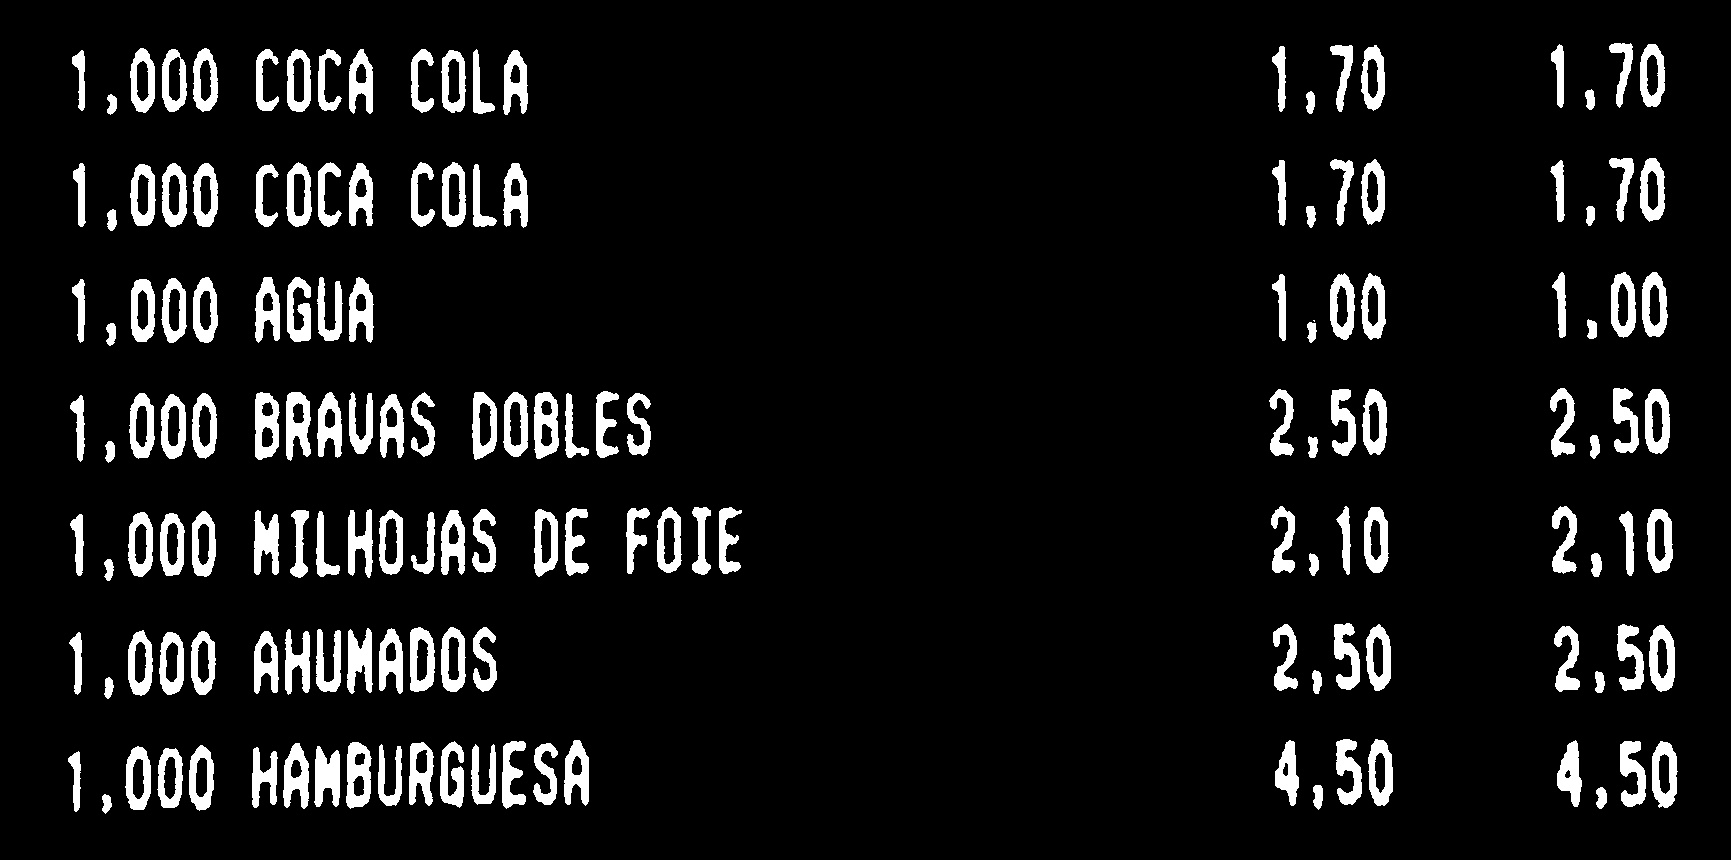
\includegraphics[width=\linewidth]{tiqueBinarizado.jpg}
			\caption{Imagen binarizada antes de dilatar}
			\label{fig:tiqueBinarizado}
	\end{minipage}
	\quad
	\begin{minipage}[b]{0.45\linewidth}
		
\includegraphics[width=\linewidth]{tiqueDilatado.jpg}
		\caption{Imagen dilatada donde se observan los rectángulos}
		\label{fig:tiqueDilatado}
		\end{minipage}
	\end{figure}

Cuando se obtienen estos rectángulos, es muy fácil conocer donde se entran las regiones que contienen las distintas lineas de productos, por ello se guarda cada linea de producto en un fichero de imagen distinto para poder después emplearlo como entrada en Tesseract.

\imagen{tiqueCortado}{Regiones de las distintas lineas de producto}

\section{Mejora de Tesseract}

Tesseract aplica por defecto su propio sistema para mejorar la imagen antes de realizar la conversión sin embargo, como se ve en \cite{improvequality}, si se aplica previamente  un algoritmo de deskewing puede mejorar la precision.

Dado que Tesseract suele cometer algún error a la hora de transformar imagen a texto, se ha desarrollado una forma de corregir las diferentes lineas de producto, para las descripción del producto se emplea  la distancia de Levenshtein(ver sección \ref{levenshtein}) aplicando un fichero de texto como soporte, es decir un diccionario, con esto se devuelve la palabra con la menor distancia, y con ello la mas parecida.

Dado que a los números de las lineas de producto no puede aplicarse una formula para corregirlos, se ha creado un fichero de concordancias por la forma del carácter que Tesseract interpreta por un número, esto se puede ver en el siguiente ejemplo:

\begin{center}
\textit{LOO REFRESCOS DE COLA 1.20 l.2U}
\end{center}

La cantidad y el importe total del la linea anterior está formada por letras y números.

\begin{table}[ht]
\rowcolors {2}{gray!35}{}
\center
\begin{tabular}{l c c c c}
\toprule
    Carácter    & Numero    \\
    \otoprule
	L 	&	1.\\
	l 	&	1\\
	O	&	0\\
	U	&	0\\
\bottomrule 
\end{tabular}
\label{tablaCsv}
\caption{Extracto del fichero de correspondencias}
\end{table}

Si aplicamos el fichero de correspondencias, podemos ver un extracto en la tabla \ref{tablaCsv}, la corrección resultante es:

\begin{center}
\textit{1.00 REFRESCOS DE COLA 1.20 1.20}
\end{center}
Con estas 2 medidas se consigue una gran mejora en las conversiones.


\capitulo{6}{Trabajos relacionados}

Se ha procedido a realizar una búsqueda de aplicaciones similares para la organización de tiques.

Las aplicaciones se han buscado en la tienda de aplicaciones Google Play de Android.

\subsection{Smart Receipts}
Smart Receipts es una aplicación que permite almacenar las imágenes de cada tique y calcular el importe total de estos.
El importe se saca de manera automática del tique, sin embargo no se tiene un desglose detallado de los artículos que se encuentran en la imagen.Como característica interesante permite exportar los datos almacenados a PDF o a un archivo CSV.

Link a la app : \url{https://play.google.com/store/apps/details?id=wb.receipts&hl=es} 

\subsection{Receipts by Wave}
Receipts by Wave permite guardar las fotos de tus  facturas, para poder ahorrarte el tener que guardar cientos de papeles.
Dispone tanto de aplicación web y móvil, sin embargo el importe total se debe añadir de forma manual.

Link a la app : \url{https://play.google.com/store/apps/details?id=com.waveaccounting.receipts&hl=es} 

\subsection{Num receipts}
Num receipt se encarga de llevar un control sobre tus gastos, el sistema funciona guardado una foto e introduciendo el importe total.
La gran ventaja de esta aplicación es su sistema de representación gráfico, que permite ver a lo largo del tiempo los gastos del usuario.

Link a la app : \url{https://play.google.com/store/apps/details?id=com.skyvin.numr.scanreceipt&hl=es} 

\subsection{Fintonic}
Fintonic es una aplicación para dispositivos Android e IOs que se encarga de llevar tus gastos personales. Su uso se basa en introducir tu cuenta bancaria y consultar los movimientos de esta.

Link a la app: \url{https://play.google.com/store/apps/details?id=com.fintonic&hl=es}

\tablaSmall{Aplicaciones relacionadas}{l c c c c}{herramientasportipodeuso}
{ \multicolumn{1}{l}{Nombre} & Escaneo Auto& Desglose Productos & Precio\\}{ 
Smart Receipts &No&No&Gratis &\\
Receipts by Wave &Si & No & Gratis&\\
Num receipts & Si & No & Gratis-Pago&\\
Fintonic & No & No & Gratis&\\
}

Como podemos ver en la tabla \ref{tabla:herramientasportipodeuso}, si que existen aplicaciones que permiten el escaneo de tiques o facturas, sin embargo ninguna realiza un desglose por productos. Estas solo permiten llevar un control de los gastos totales por factura, lo que limita al usuario saber que ha consumido a menos que consulte la foto que realizo al tique.

Una aplición curiosa es el caso de Menta\cite{menta} la cual es una aplicación de descuentos.
Su funcionamiento es muy simple, cada día hay una serie de productos en oferta, si has adquirido dicho producto, con hacerle una simple foto, el sistema detecta si el producto se encuentra en la imagen.





\capitulo{7}{Conclusiones y Lineas de trabajo futuras}
\subsection{Conclusiones}
Las conclusiones que se pueden extraer del desarollo del presente trabajo pueden resumirse en:
\begin{itemize}
	\item Se ha obtenido una aplicación funcional, que a partir de una imagen de un tique se obtienen los diferentes artículos adquiridos. Hasta donde se conoce, este es el primer sistema de este tipo. Dado que se trata  una primera versión, existe mucho margen de mejora para futuras versiones, como se describe en \ref{lineasFuturas}.
	\item Debido al uso de varios campos para desarrollar el trabajo, se han utilizado una gran cantidad de conocimientos adquiridos en la carrera, y sobre todo nuevos campos como son la visión artificial junto con OpenCv y el desarrollo de aplicaciones bajo el Sistema Operativo Android.
\item Un aspecto muy relevante que se ha sacado de este proyecto es el desarrollo del mismo, de como a pesar de llevar una planificación pueden surgir imprevistos que pueden ayudar o entorpecer el desarrollo del mismo.
\end{itemize}

\subsection{Lineas de trabajo futuras \label{lineasFuturas}}
Este proyecto representa una version inicial de una aplicación que debe evolucionar y ampliar sus funcionalidades.

Durante la fase de diseño se ha tenido muy en cuenta la realización de una aplicación que permita posteriores ampliaciones y mejoras. Se ha buscado crear una base sobre la que se pueda seguir como referencia a la hora de realizar trabajos parecidos o ampliar el mismo. Ha habido algunas ideas que no han podido ser incorporadas debido a la falta de tiempo, y que podrían ser implementadas en un futuro. A continuación se proponen algunas:

\begin{itemize}
	\item \textbf{Ampliación del tipo de tique:} A día de hoy, la aplicación solo se ha diseñado para funcionar con un solo tipo de tiques, sin embargo, lo ideal seria utilizarla con varios modelos para alcanzar un número de productos y establecimientos superior.
	\item \textbf{Categorización automática:} Durante la realización del proyecto, se estudio como poder categorizar los productos automáticamente, se ha estudiado la herramienta BabelNet, la cuál es una base de datos semántica, que relaciona algunas palabras  con su significado como por ejemplo pan:con alimento o algunas marcas con la compañía como San Miguel con cerveza. El principal inconveniente es que cada tipo de entidad tiene muchos atributos diferentes y usarla sería muy complicado.
	\item \textbf{Utilización de la Minería de datos:} Usando word2vec una palabra se transforma en un vector, este conserva la semántica original, por lo tanto vectores próximos entre si pertenecen a la misma categoría y están alejados de otros vectores que provienen de palabras que entrarían en otra categoría, Si vemos la imagen \ref{fig:vecinos}, las zonas rojas podrían corresponder a la categoría de carnes, mientras que la zona azul seria la categoría pescados.En función de donde el algoritmo sitúe la palabra de la que se desea conocer la categoría, la categoría seria una u otra.
	\imagen{vecinos}{Gráfico de vecinos mas cercanos}
	
	\item \textbf{Nuevas características:} Dado que los productos son almacenados en un sistema persistente, es posible realizar una base de datos global, nutrida por todos los clientes, lo que supondría un conocimiento preciso de los productos y precios de estos en cada momento, y por lo tanto realizar búsquedas de dónde se localizan los productos con menor coste en tiempo real. Sin embargo establecer una relación entre los productos que simbolizan lo mismo pero con nombres diferentes, desembocaría en un coste elevado.
\end{itemize}

\nocite{*}
\bibliographystyle{plain}
\bibliography{bibliografia}

\end{document}